%!TEX root = hcwsa.tex

\chapter{初来乍到}\label{chap:初来乍到}

  本章主要分为八个部分:

  Sec \ref{sec:银行} 银行的\textsbf{开户} (入境德国前) 和\textsbf{激活} (入境德国并获得常住地址后),以及在亚琛较为广泛使用的三个银行——德意志银行、亚琛储蓄银行 (Sparkasse Aachen) 和 N26 的业务办理的异同;

  Sec \ref{sec:医疗保险} 医疗保险,包括\textbf{私立医保} (用于递签,在入境德国前办理) 和\textbf{公立医保};

  Sec \ref{sec:住房} 住房的相关事宜;

  Sec \ref{sec:申请签证及入境} 申请签证和入境前往亚琛;

  Sec \ref{sec:重要事务办事点} 是对大学市政厅、SuperC、外管局三个重要办事点的介绍 (因为历史和地理原因,导致在描述这些地点的时候往往采用不同的词,以致给新生造成混乱,特此澄清);

  Sec \ref{sec:入境两周内必办事宜} 将覆盖入境后两周内要办的事情:购买电话卡和办理宽带,户口登记/Anmelden,银行账户激活,申请\textbf{公立医保}用于入学注册;

  Sec \ref{sec:RWTH注册和管理系统} 涉及入学注册、初步接触学校的学生管理系统以及使用其邮箱;

  Sec \ref{sec:申请居留许可} 申请居留许可的一系列事宜和 FAQ。

  入境前要办的事情有:银行\textsbf{开户}(Sec \ref{sec:银行})、申请\textbf{私立医保}用于递签 (Sec \ref{subsec:私保申请和缴费}) 和寻找住房 (Sec \ref{sec:住房})。这些事情在RWTH发Zulassung后就可以着手办理。银行账户的\textsbf{激活} (领取银行卡用于消费) 和申请\textbf{公立医保}则是在入境德国\textbf{并有了常住地址}之后办理的。

  \textsbf{Anmelden} 作为一个关键概念须在本章引言部分提出。Anmelden是德语中 ``(户口)登记''\footnote{有的论坛里用的词叫``落户''。}的意思,简称 \textsbf{An}。类似的一个词是 \textsbf{Abmelden},``(户口)注销''。在德国境内居住的德国人和外国人都有登记户口的义务。Anmelden 手续是凭\textsbf{住房合同}到当地市政厅办理的,完成后您将现场拿到一张\textbf{纸质证明},证明您在当地\textbf{有固定住所}。有了 \textsbf{Anmelden 的纸质证明},您才可以办理银行业务、消费、公立医保申请、入学注册等事情。

\section{银行}\label{sec:银行}

  外籍学生都必须使用德国境内的银行进行消费,它是申请德国签证必需的材料之一;此外,银行的选择涉及到在当地消费的便捷度。

  为使概念明晰,我们把银行的\textsbf{开户}和\textsbf{激活}都放在这里介绍,尽管激活是入境后才需要去办的事情。

  \subsection{概念澄清}\label{subsec:概念澄清}
 
    德国有不少银行都支持在国内办理\textsbf{开户/Account Opening},适用于留学生且便于在亚琛生活的银行有\href{https://www.deutsche-bank.de/pk.html}{\textsbf{德意志银行/德银/Deutsche Bank/DB}} (后文用德银指代)、\href{https://www.sparkasse-aachen.de/de/home.html}{\textsbf{亚琛储蓄银行/Sparkasse Aachen}} 和 \href{https://n26.com/en-de/free-bank-account}{N26}。

    用于\textbf{申请德国签证}所开通的德国境内的银行账户是指\textsbf{冻结账户/Blocked Account/Sperrkonto},存入的资金叫\textsbf{冻结资金/Blocked Balance/Sperrbetrag}。词缀\textsbf{冻结/Blocked/Sperr-}指的是开户人在前往德国之前\textbf{不得使用}该账户内的资金,这是德国出于涉外金融安全的考虑,因此\textsbf{Sperrkonto}也被称为\textsbf{限制提款账户} (``冻结''和``解冻''等字样也出现于签证相关的文件里)。\textsbf{Sperrbetrag}也称\textsbf{自保金},每月提款额度不得超过一定金额,如934欧。所规定的这934欧是最基本的生活保障,是为了保障留德学生有足够的资金维持在当地一年共计11,208欧的生活费用\footnote{当然,您还可以通过其他方式获得更多的生活费。所以934欧并不是固定的,在开户表格上可以自行决定。}。这个数额是德国政府基于在德大学生的消费调查而规定的,相对稳定,不随利率波动\footnote{2018年的自保金数额是8,640欧,这个数额已沿用多年,2020年的数额是10,236欧,2023年的数据是11,208欧。}。

    用于\textbf{日常消费} (含伙食、支付房租、支付学期费、后续接受父母资助等) 的银行账户称为\textsbf{借记账户/Debit Account/Girokonto}。每一个留德学生的名下都有 Sperrkonto 和 Girokonto,\href{https://china.diplo.de/blob/1341652/c79bd5edf0554386e9c4285bd447c2fc/pdf-merkblatt-natvisum-studium-data.pdf}{Sperrkonto} 的作用仅仅是用于首次申请前往德国的签证,以及在德的第一年里,\textbf{Sperrkonto每月自动把一定数额的欧元 (1,027欧) 汇入到 Girokonto},即每月月支出不得超过12,324欧;第一年以后,Sperrkonto的钱用完了,接受父母资助的账号是 Girokonto 的 IBAN,而不是 Sperrkonto 的IBAN。

    在转账场合 (如支付学期费和接受父母资助) 都需要 \textsbf{IBAN} 和\textsbf{BIC}。IBAN 用于标识欧元区域内的银行账户,格式为``DE+20位数字'';BIC 是银行识别码,也称为SWIFT代码,跟银行分行有关,跨境汇款中,BIC 确保汇款能够到达正确的银行和分支机构。此外,欧盟的银行系统里对\textsbf{账户号/Konto-Nr/IBAN}和\textsbf{卡号/Karten-Nr}是有区分的。\textsbf{Karten-Nr}的具体格式取决于银行。这种设计是为了防止卡遗失\footnote{挂失后新发的卡的Karten-Nr跟旧卡的Karten-Nr不一样,但他们的IBAN是一样的。}。Fig \ref{fig:德银、Sparkasse Aachen 和 N26 的 IBAN 和 BIC} 展示了三家银行的相关信息。Sperrkonto 和 Girokonto 都有对应的 IBAN 和 BIC, 然而 \textbf{Sperrkonto 是不发卡的,Girokonto 则会发对应的 Girocard}。

    \begin{figure}[t]
      \centering
      \begin{minipage}{.35\textwidth}
      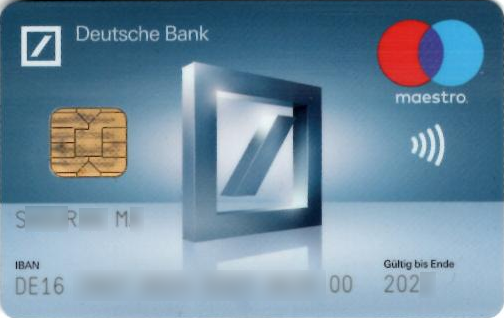
\includegraphics[width=\textwidth]{初来乍到/Bank/DB1.png}
      \vskip.5\baselineskip
      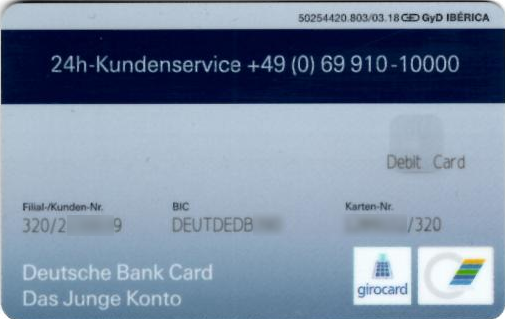
\includegraphics[width=\textwidth]{初来乍到/Bank/DB2.png}
      \end{minipage} \ 
      \begin{minipage}{.35\textwidth}
      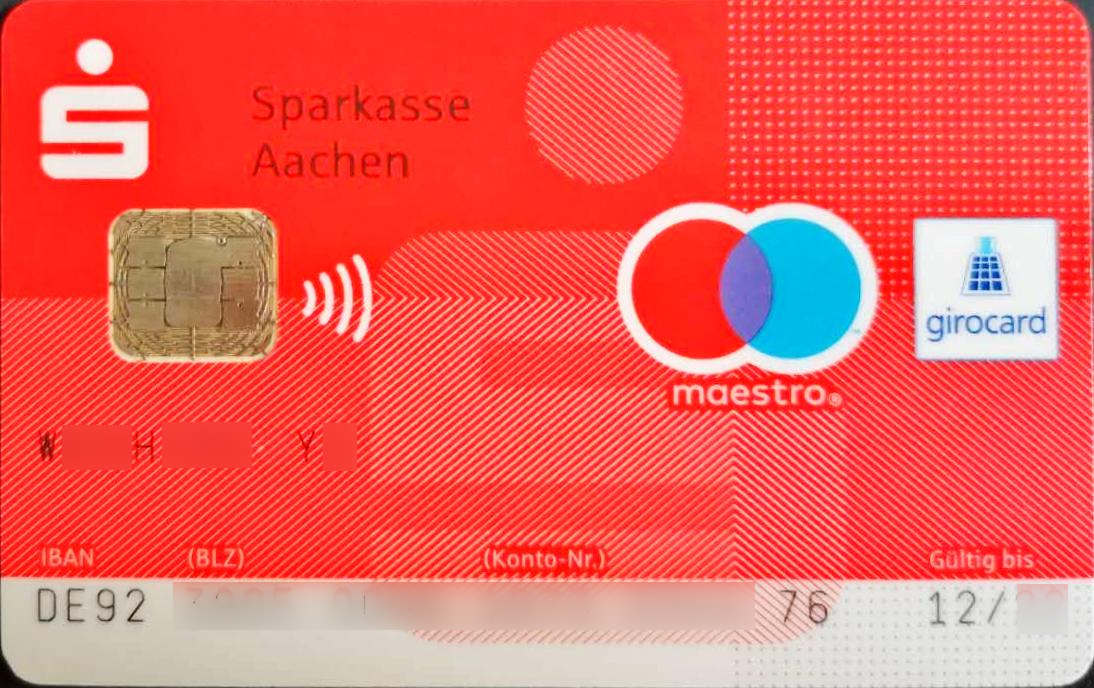
\includegraphics[width=\textwidth]{初来乍到/Bank/Sparkasse1.png}
      \vskip.5\baselineskip
      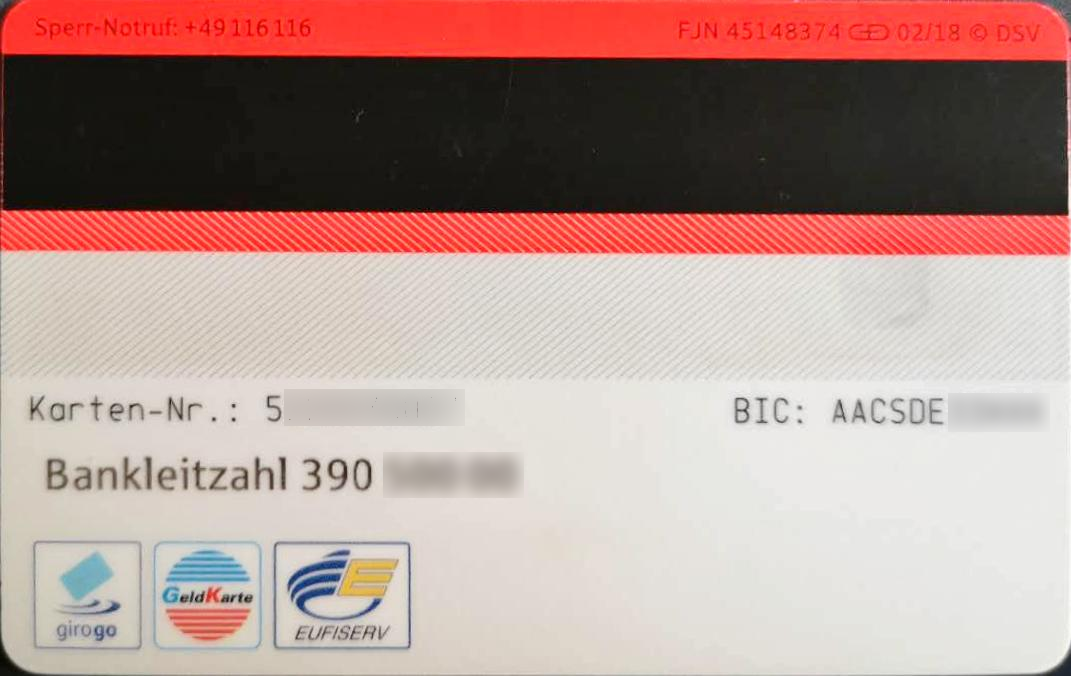
\includegraphics[width=\textwidth]{初来乍到/Bank/Sparkasse2.png}
      \end{minipage} \ 
      \begin{minipage}{.2\textwidth}
      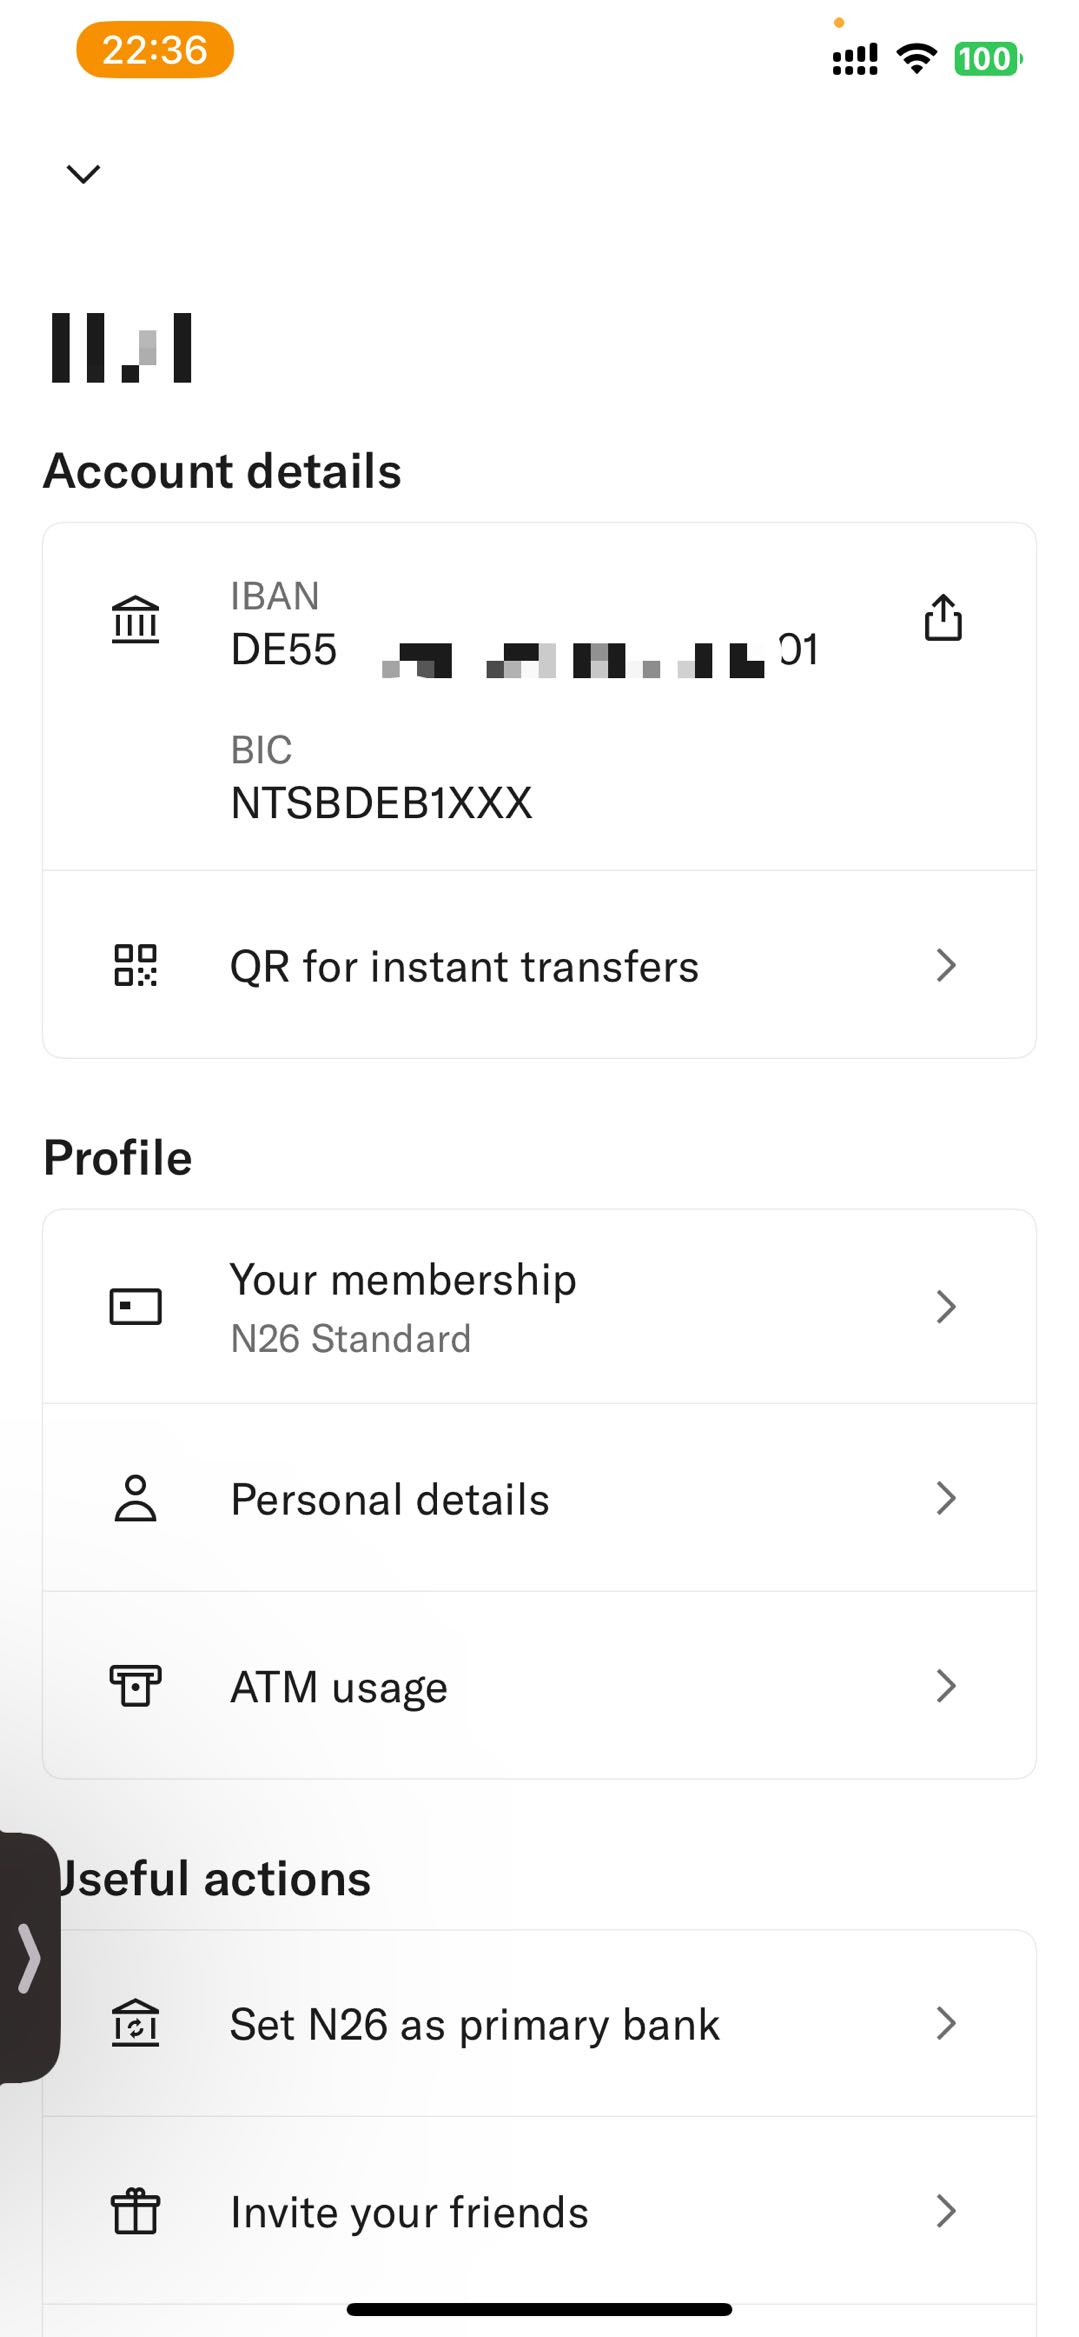
\includegraphics[width=\textwidth]{初来乍到/Bank/N26.jpg}
      \end{minipage}
      \caption{德银、Sparkasse Aachen 和 N26 的 IBAN 和 BIC}
      \label{fig:德银、Sparkasse Aachen 和 N26 的 IBAN 和 BIC}
      \vskip-\baselineskip
    \end{figure}

    银行系统有\textsbf{借记卡/储蓄卡/Debit Card/Girocard} (不可透支) 和\textsbf{贷记卡/信用卡/Kreditkarte} (可透支) 两种类型的账户的区分。借记卡和贷记卡是书面语,储蓄卡和信用卡是口语。由于货币的结算方式不同,银行规定,借记卡只能用于发卡行的境内消费,而贷记卡则可以用于国际消费,以特定的结算方式计入到发卡行所在国的持卡人的借记卡上。\textsbf{银联/UnionPay}、\textsbf{VISA}、\textsbf{MasterCard/万事达}是不同贷记卡所采用的不同的结算方式。Sparkasse Aachen 在信用卡的业务上推行了不少福利,在办理 Girokonto 激活业务的同时会推荐办理其贷记卡。

    关于这两个账户跟三个银行的关系见Table \ref{table:Sperrkonto,Girokonto}。

    \begin{table}[ht]
      \centering
      \vskip-\baselineskip
      \caption{Sperrkonto \& Girokonto 和三家银行的关系}
      \begin{tabular}{|c|c|c|}
      \hline
      &Sperrkonto&Girokonto\\
      \hline
      德银&\multicolumn{2}{c|}{同一个IBAN}\\
      \hline
      Sparkasse&IBAN for Sperrkonto&IBAN for Girokonto\\
      \hline
      N26&\multicolumn{2}{c|}{同一个IBAN}\\
      \hline
      \end{tabular}
      \label{table:Sperrkonto,Girokonto}
      \vskip-\baselineskip
    \end{table}

  \subsection{德意志银行}\label{subsec:德意志银行}

    \textbf{德意志银行}的\textbf{开户}流程如\href{https://china.db.com/china/company/downloads/}{这里}所示:

    \begin{enumerate}
      \item 从\href{https://www.deutsche-bank.de/pfb/content/pk-konto-und-karte-international-students.html?pfb_tab=34880-34883}{官网}下载申请表格并且填写。默认 1,027 欧的每月提款额度可以填写其他数额。
      \item 前往德银驻北/上/广分行办理相关材料,并将拿到\textsbf{个人编号通知单}。
      \item 根据\textsbf{个人编号通知单}的信息汇款。该通知单上有两个收款账号:一个是德银总部的负责相关业务部门的 IBAN,汇款的 12,324 欧是\textsbf{自保金};另一个是 德银驻华分行的工作人员的账号,汇的是手续费。
      \item \textbf{先后}收到来自德银驻北/上/广分行的两份\textbf{纸质信函},分别是\textsbf{存款证明}和\textsbf{开户证明/Kontoeröffnung}。后者有您的IBAN。
    \end{enumerate}

    至此,德银的\textsbf{开户}流程办理完毕。下面是\textsbf{激活}流程:

    \begin{enumerate}
      \setcounter{enumi}{4}
      \item 入境德国,获得长居住房合同,Anmelden,得到相关的证明,上面有您在德国的长期住址。
      \item 在\href{https://www.deutsche-bank.de/pk/konto-und-karte/konten-im-ueberblick/internationale-studenten1.html#parsys-tabs_copy_1250445051-tabsParsys-tabpanel_1536556080-tabPanelParsys-accordion-accordionParsys-accordionentry_317017862}{官网\MVRightarrow{} Activate a blocked account}下载表格填写,打印,签字。街头的打印店有\textsbf{unicopy}。
      \item 邮寄给汉堡办事处,网上搜索\textsbf{Deutsche Post}可知邮筒的位置。不必去\textsbf{德银驻亚琛支行/Deutsche Bank Filiale Aachen}。
      \item 大约一周以后,您会收到来自德银的若干封\textbf{纸质信件},包括但不限于网银密码 (\textsbf{Online-PIN})、Girocard和卡密码 (\textsbf{Geheimzahl})、photoTAN (德国版的网银支付二维码) 的激活码,等等。
    \end{enumerate}

  \subsection{Sparkasse Aachen}\label{subsec:Sparkasse Aachen}

    德银的开户流程有个硬伤是,您须前往德银驻华分行办理业务;此外在亚琛生活,德银的 ATM 机仅市中心的\textsbf{德银驻亚琛支行/Deutsche Bank Filiale Aachen}一家。相较之下,Sparkasse Aachen 在全亚琛有大大小小的 ATM 机以及银行服务点,取钱和办理各种银行服务较为方便。

    Sparkasse Aachen 的办理流程如\href{https://www.sparkasse.de/pk/ratgeber/bildung/studium/sperrkonto.html}{这里}所示。发邮件即可完成基本的办理:

    \begin{enumerate}
      \item 根据如下模板发邮件给 \href{mailto:896-visa@sparkasse-aachen.de}{896-visa@sparkasse-aachen.de} 告知银行的工作人员说您要开通Sperrkonto。附件为\textbf{大学录取通知书}和\textbf{护照}。
    \end{enumerate}

    \vskip.5\baselineskip
    \noindent\fbox{
      \begin{minipage}{\textwidth}
        Betreff: Sperrkonto/ blocked account

        Sehr geehrte Damen, sehr geehrte Herren,

        Dear Sir or Madam,

        \vskip1em

        Als zukunftige Studentin einer Hochschule in Aachen mochte ich bei der Sparkasse Aachen ein Sperrkonto einrichten.

        As a future student at one of the universities in Aachen, I would like to create a blocked account at Sparkasse Aachen.

        \vskip1em

        Die Bestatigung liber den Studienplatz der Hochschule und eine Passkopie habe ich als Emailanhang beigefiigt.

        The confirmation of acceptance at the university and the passport copy is attached.

        \vskip1em

        Viele GruBe

        Kind regards

        Vorname Nachname
      \end{minipage}
    }
    \vskip.5\baselineskip

    \begin{enumerate}
      \setcounter{enumi}{1}
      \item 工作人员回复,让您汇款给 Sparkasse Aachen 的 Sperrkonto,以及提供您的地址和电话等资料。 
      \item 收到\textsbf{存款证明}和\textsbf{开户证明/Kontoeröffnung}这两个文件的\textbf{纸质信函}和\textbf{Email}。
    \end{enumerate}

    至此,Sparkasse Aachen 的\textsbf{开户}流程办理完毕。下面是\textsbf{激活}流程:

    \begin{enumerate}
      \setcounter{enumi}{3}
      \item 入境德国,获得长居住房合同,Anmelden,得到相关的证明,上面有您在德国的长期住址。
      \item 打电话约 Termin,届时带上护照和 Anmelden 的证明前往 Sparkasse Aachen Filiale 办理 Sperrkonto 的激活以及 Girokonto 的开户和激活。在 Girokonto 的开户表格上确定每月提款额度。
      \item 收到网银密码、Girocard和卡密码。
    \end{enumerate}

    值得一提的是,Sparkasse Aachen 提供的 Girokonto 服务比较多样,如\href{https://www.sparkasse-aachen.de/de/home/privatkunden/girokonto/s-pool.html}{\textsbf{S-POOL Konto}}。这是 Sparkasse Aachen 专门为18-30岁的学生准备的青年账户。只需要出示有效的学生证明,办理 S-POOL Konto 的账户时即可享受优惠的账户管理费。办理 S-POOL 账户时,还可以选择免费申请一张 Mastercard,对于买机票住酒店等大额消费来说非常的方便。此外,S-POOL 账户还和亚琛的诸多商家有合作,付款时使用 S-POOL 卡能够享受优惠。相较德银来讲,Sparkasse Aachen 是在亚琛学习和生活的首选。

  \subsection{N26}\label{subsec:N26}

    由于德银和 Sparkasse Aachen 的 Girokonto 的激活都须要德国的常住地址,这对于刚入境的留学生而言是比较不友好的。后起之秀 \href{https://n26.com/en-de}{N26} 为此提供了更好的解决方案:其激活并不需要 Anmelden。

    N26 的开户和激活能在小红书、知乎等大部份华语社区里找到经验贴。跟 Sparkasse Aachen 一样,N26 的开户流程也基本上是在线上解决,稍微不一样的一点是,N26 的开户需要提供一个\textbf{德国境内的地址} —— 这可以是您的一个住在德国的朋友的地址。按提示完成了开户手续以后,您即可凭相关证明去递签,同时 N26 会给您的朋友寄送 Girokarte 等证件。入境了德国,从朋友那里拿到了 Girokarte 并修改密码,就算是激活成功了。

\section{医疗保险}\label{sec:医疗保险}

在德国大学生必须购买\textsbf{医疗保险/Krankenversicherung}。医疗保险公司有\textsbf{公立保险/法定医疗保险}和\textsbf{私立保险}之分,也就是我们俗称的\textsbf{公保}和\textsbf{私保}。通常情况下,在入境之前无法办理公保 (例如短期签证不需要、\textbf{没有德国境内的固定地址}、银行账户没办好等等),所以办理的私保则只用于递签;当您有了在德固定地址以后,才可以申请公保。

  \subsection{私保申请和缴费}\label{subsec:私保申请和缴费}

    最终完成学校的申请须提交私保的开通证明。私保的选取大同小异,跟公保公司AOK合作的私保是Klemmer。按邮件的指引签署扣款协议,钱就从您的在国内银行的贷记卡中扣除。这就完成了``入境德国180天有效、直到法定医疗保险生效''\footnote{\href{https://china.diplo.de/blob/1341652/cd1526772cd3d64a3f122f07d908a16b/pdf-merkblatt-natvisum-studium-data.pdf}{德国驻华使领馆\MVRightarrow{} 服务\MVRightarrow{} 签证和入境\MVRightarrow{} 长期停留\MVRightarrow{} 留学签证申请须知}} 这段时间内的医保扣款。

  \subsection{公保申请}\label{subsec:公保申请}

    一般的留德学生都会选择公保,公保的保险公司也有很多,\href{https://www.aok.de/}{AOK} (有\href{http://www.aok-cn.com/}{中文网站},位于Ursulinerstraße的门店如 Fig \ref{fig:亚琛的 AOK 门店} 所示),\href{https://www.tk.de/techniker}{TK} (在亚琛的门店较 AOK 更多),DAK 等等,每个月的保险费在123欧左右。持语言签证的学生只能选择私保,每月保险费28欧起。来德国高校的交换生也推荐私保,因为此时私保的价格相对于公保要更便宜。

    办理公保所需的材料包括:护照、银行帐号、录取通知书,具体如 Sec \ref{subsec:医保激活} 所述。在高校注册入学时,需要出示医疗保险证明,可以向医疗保险公司索取。公保的缴费是每月从IBAN中自动扣除的。

    若您选择Klemmer,则当您有了Anmelden的证明、并按邮件指引进一步更新了住址的同时,该公司就帮您同时申请了AOK公保;当然您也可以选择仅扣款,而公保则自己找心仪的公保公司。

    \begin{figure}[ht]
      \centering
      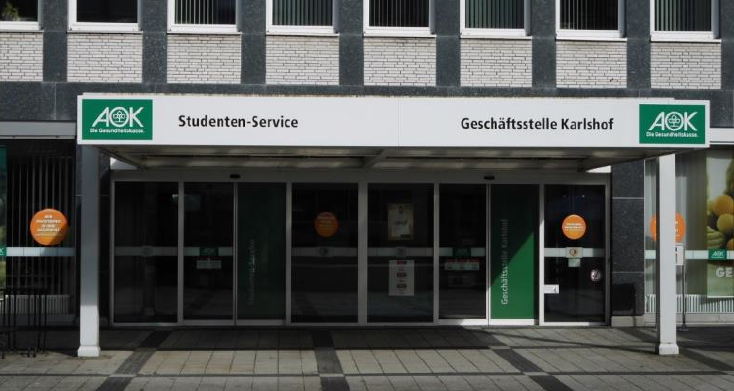
\includegraphics[width=.5\textwidth]{初来乍到/AOK.jpg}
      \caption{亚琛的 AOK 门店}
      \label{fig:亚琛的 AOK 门店}
      \vskip-\baselineskip
    \end{figure}

\section{住房}\label{sec:住房}

  亚琛在9月到11月期间,房源会变得异常紧俏。为了在初到亚琛之际能有一个落脚点,建议您尽可能通过多种渠道去寻找房源,先找个可以 Anmelden 的房子落脚,等找房高峰过去并初步熟悉当地环境以后,再慢慢寻觅符合自己需求的房源。

  \subsection{住房形式}\label{subsec:住房形式}

    德国高校的\textsbf{大学生服务中心/Studentenwerke}为学生提供了一系列的服务,从大学的\href{https://bewerberportal.stw.rwth-aachen.de/}{租房网页}上可以概括性地了解相关信息,如水电暖网以及房屋内景等。

    其次有由房屋公司提供的\textsbf{公寓}或者房东是当地人的\textsbf{私房}。``公寓''在国内语境不难理解,而``私房''则往往意味着会有同居的室友,这种情形也描述为``您跟您的室友\textsbf{WG}一个房子''。因为在德国,很常见的一类房子是长这样的:它是某个小楼的某一层中的其中一间\textsbf{Wohnung},进去后是2\textasciitilde3个\textsbf{小房间/Zimmer}租给不同的租客,公用厨房 (厨具最好用自己的;若自己当前租的房子是zwischen的话就用二房东的)、厕所和冲凉房。洗衣机可以是在冲凉房内、地下室里,或者公寓附近。

    一个可An房只允许单人居住,除非能提供结婚证才可允许夫妻同居。

  \subsection{租房信息}\label{subsec:租房信息}

    在亚琛寻找房源主要有以下渠道,通常前两个是最稳妥最常用的:

    \begin{itemize}
      \item 学生公寓:所有宿舍的申请入口\href{https://bewerberportal.stw.rwth-aachen.de/}{汇总}。申请学生宿舍一般会有一段较长的排队等待时间。
      \item 中文社群:微博、QQ群、微信群、小红书。作为一座大学城,亚琛的房源流动性很强,也由此有很多本地找房微信群。添加亚琛学联小助手 RWTHChina 进入新生群可获取及时的资讯。
      \item 德语网站:\href{http://www.wg-gesucht.de}{WG-Gesucht.de} \& \href{http://www.studenten-wg.de}{HousingAnywhere} \& \href{https://www.immobilienscout24.de/}{ImmoScout24} (充值为会员的话回复概率大)。
      \item 私人学生宿舍:这个\href{http://www.stwkhg.de/}{教会宿舍}有多栋学生宿舍;\href{https://www.esg-aachen.de/}{ESG Aachen}位置优秀,离学校仅大约数分钟步行路程。\href{http://www.t39.rwth-aachen.de/}{Templergraben 39}是学生自治宿舍。
      \item 布告栏:Mensa,Audimax,Mogam等自习室的信息栏。
    \end{itemize}

  \subsection{租房合同和注意事项}\label{subsec:租房合同和注意事项}

    在德国,签订住房合同是一件很慎重的事情,签字之前务必仔细阅读住房合同。一份合同的有效期通常是一年,为双方省事,一年满后默认续签;需要特别注意的是租房合同中与扣取押金及解除合同后押金返还有关的条目,不清楚的需要向房东详细询问。

    德国租房分\textsbf{冷租/Kaltmiete} 和\textsbf{暖租/Warmmiete} 两种。暖租即房租中包括了\textbf{水电暖、网费}、管理费等费用,冷租则需要去水电公司自行办理,水电公司可以通过Check24寻找最优惠的。若不包网费,得自行去运营商门店办理宽带 (Sec \ref{subsec:电话卡和宽带})。

    有了德银的IBAN码,是可以在没有收到银行卡的情况下签订房租的自动扣款合同的。

    敲定以上事宜后,房东会草拟一份合同抄送给您,但这份合同并未经您签字。在入住和签订合同之前,房东会带您在房间里查看一圈,清点家具并检查房间的损坏程度。签了字,并按要求付了\textsbf{押金/Kaution} (通常为房租月租的1\textasciitilde3倍) 之后,您就是房间的主人了:倘若以后有物品损坏,会被扣押金。

    房东交给您的钥匙一定要保管好,因为在德国,很可能一层楼都用同一把钥匙开门。一旦钥匙丢了,房东很可能会把一层楼的锁都换掉。这个风险不可能通过私自配钥匙避免,因为在德国配钥匙需要房东和警察局的双重证明到专门的店里去配才行。

    如果您要换房,可以以提前找好续租者/下一任房客/Nachmieter的方式提前结束租房合同。否则,须提前三个月提前通知房东以解约。

    拿到合同并An了之后记得在自己的门牌上贴上自己的名字,或要求房东更换公寓楼下的住户列表,确保快递员和信使找得到您的名字。同时,\textbf{记得到RWTHonline更新地址},以免学校寄给您的纸质信件丢失。

  \subsection{租房广告里的常见名词之定义}\label{subsec:租房广告里的常见名词之定义}

    鉴于微信群是目前最有效的房源,我们特地把租房广告里常见的名词缩写加入在此,因为这些名词经常出现在租房广告里。

    \textsbf{An}: Anmelden的缩写。微信群的租房广告中常把Anmelden简称An。

    \textsbf{房东/房主}:房屋的产权人,合同中的乙方。

    \textsbf{二房东/Untervermieter/出房人}:往往是在这里就读了一段时日或者是即将毕业的学生。ta跟房东签订了合同并有该房子的Anmelden证明。

    \textsbf{租客/续租者/下一任房客/Nachmieter}:就是读者,``您''。

    \textsbf{可An房}:二房东须解除ta自己的租房合同并去\textsbf{市政厅/Bürgerservice} (Sec \ref{subsec:市政厅 Bürgerservice Katschhof} \& Sec \ref{subsec:签订住房合同以及Anmelden}) 退注册,ta因为毕业或者是找到了更好的房子需要搬家故把旧房转出。同时您要跟房东签署您自己的租房合同并去Bürgerservice拿Anmelden证明。

    \textsbf{Zwischen房/不可An房/临时住房}:二房东不解除合同,不去Bürgerservice退注册,ta仅仅是实习或者假期回国导致房子闲置所以出房,中间的这一两个月给租客来住,从而填补这一两个月的租金。租客也因此不必跟房东签合同,但会跟二房东签订一份形式上的合同 (私下商定)。

    \textsbf{WG}:即Wohngemeinschaft,合租。

    \textsbf{Wohnung \& Zimmer}:Zimmer $\in$ Wohnung。譬如在租房广告里常见的表述:5 Zimmer Wohnung。

    \textsbf{Nach}:即\textbf{家具转出}。通常房子的家具都能留下给下一个租客,出钱买或者不出钱买只是租客跟二房东私下商定;若租客是去一些公司管理的公寓直接找房或者是排到学校公寓的话,这个房子往往是空房,没有家具,得自己买,比较麻烦。

    \textsbf{押金/Kaution}:搬入时需交纳,通常为房租的1-3倍,需要特别注意的是租房合同中与扣取押金及解除合同后押金返还有关的条目,不清楚的需要向房东详细询问。

    \textsbf{定金}:\textbf{跟押金经常混用}。在租客表达了入住意向且房东也有意向将此房出租给此租客 (因此需要把租房广告撤回) 的情况下,由于某种原因 (如不确定入住日期等) 无法及时签订合同,因此会用 (通常不超过100欧的) 定金的方式作为一种\textbf{私下的信用协商}。但是须注意,这种方式\textbf{没有保护效益},交定金前要慎重。

  \subsection{出境前寻找住房的注意事项}\label{subsec:出境前寻找住房的注意事项}

    因为您此时在国内而房东在国外,所以这里列出\textbf{在出境前}寻找和确定住房需要注意的点:

    \begin{enumerate}
      \item 最好是选择\textbf{可以Anmelden的房子},可以是大学学生宿舍、当地公寓或私房,这样您能在到达亚琛的一个月内签订合同,并进而办理Anmelden手续、银行账户激活和公保申请 (Sec \ref{sec:入境两周内必办事宜})。如果房子是临时住房,也一定要尽快确定可以An的房子,否则生活会有很多不便利。
      \item \textsbf{大学学生公寓最}为方便省事,因此它是大部分学生的首选,这也意味着申请人数众多。只要提前足够长的时间\href{https://bewerberportal.stw.rwth-aachen.de/}{申请},就有很好的机会拿到学生宿舍的房间。因此通常申请大学的同时就申请学生宿舍。
      \item 对于在微博或者微信群里找到的私房 (\textsbf{二房东}通常是中国人),可以通过视频实现在线看房,技术上不是难度。如果双方谈妥,可以先交\textsbf{定金},这样一到亚琛就可以办理签合同事宜。
      \item 须关心住所跟学校、学院、上课地点的相对位置,以便节省通勤时间。
    \end{enumerate}

\section{申请签证及入境}\label{sec:申请签证及入境}

  有了前三章的铺垫,申请签证就水到渠成。从国内到亚琛市通常包含三步:购买机票入境,从入境城市乘坐列车到达亚琛,从车站乘公交到住所。

  \subsection{签证申请}\label{subsec:签证申请}

    签证前通常要完成的事情包括APS面谈,学校申请,(CSC申请),银行开户和医保申请。因为已经有了APS证书,所以签证是免面试的,所要做的是到德国驻华使领馆提交签证申请表即可。递签的流程和所需材料皆可在\href{https://china.diplo.de/cn-zh/service/visa-einreise/nationales-visum/1345434?openAccordionId=item-1345454-4-panel}{德国驻华使领馆\MVRightarrow{} 服务\MVRightarrow{} 签证和入境\MVRightarrow{} 长期停留}上找到。

    注意到所填的``预计进入申根区日期'',这意味着您在递签之前要确定好自己的机票。关于订机票的事宜详见下一小节。

  \subsection{购买机票入境}\label{subsec:购买机票入境}

    从携程、飞猪等中间商,或者从航空公司网站 (汉莎航空是德国最大的航空公司) 直接查询并购买机票。通常的目的地是杜塞尔多夫或者法兰克福。两个城市都有其优劣:杜塞尔多夫跟亚琛都在北威州,火车频次多,几乎不用转车,但航班班次相对较少;法兰克福是德国的经济重镇,航班班次较多,但入境查个人物品比较严格。

    \textbf{入境时间}跟\textbf{开学时间}不要相差太短但也不必太长。大约两周左右即可搞定 Sec \ref{sec:入境两周内必办事宜} 和 Sec \ref{subsec:入学注册} 的所有事情。

    初次入境会比较多地考虑行李限额。\textbf{部分航空公司对留学生有行李优惠},能以经济舱的票价享受托运大件行李 (包括托运行李的个数以及总重) 的权利。具体须向航空公司咨询。

    特别强调通讯网络的重要性,尤其是当您踏上异国的土地的时候,手机没有网,是寸步难行的。建议在国内淘宝购买欧洲旅行专用的\textbf{电话卡} (通常一个月失效,但已足够时间在德国买一个新的,见 Sec \ref{subsec:电话卡和宽带}) 。

  \subsection{从入境城市乘坐列车到达亚琛}\label{subsec:从入境城市乘坐列车到达亚琛}

    从Deutsche Bahn (DB) \href{https://www.bahn.de/}{官网}或其 \href{https://www.bahn.de/p/view/service/mobile/db-navigator.shtml}{App (DB Navigator)} 查询列车班次并线上购买车票即可 (需信用卡或 PayPal)。保存在个人移动设备上 (无需打印) 即可应对查票。火车站 DB 自助机或柜台也可直接购买车票,自助机一般不接受信用卡和 100欧以上的大额纸币。

    关于\textbf{出发地},通常都会选择当地的主火车站 (Hauptbahnhof)。名字里带个Hauptbahnhof的是每个城市的大站,比较多列车班次。考虑到部分城市的机场和火车站的距离并不很近得靠机场巴士接应,并考虑到在机场取行李的时间,不建议在起飞前就订好车票。而且列车是班车,无需担心一天只有一班的情形。

    亚琛共四个火车站可作为\textbf{目的地}:\textsbf{Aachen Hbf},\textsbf{Westbahnhof},\textsbf{Schanzbahnhof},\textsbf{Rothe-Erde Bahnhof}。可以选择离住所近且可以直达的火车站下车。通常Aachen Hbf是首选。

    法兰克福直达亚琛的车次一般为高速动车 (ICE),其车次较少。建议乘ICE至科隆后,在科隆转乘RE或RB\footnote{州内短途列车/区域快车/Regional Express (RE)/Regionalbahn (RB)。见 Sec \ref{sec:交通}。}。从杜塞前往亚琛可以乘RE直达。

  \subsection{从车站乘公交到住所}\label{subsec:从车站乘公交到住所}

    可从\href{http://www.avv.de/}{AVV官网}或其\href{http://www.avv.de/}{App (AVV connect)}或上网查询线路。Google Map的线路足够可用。AVV也是在亚琛生活必不可少的app,除了线路之外可以用来查询公交到站时间。

    最直接的购票方式是在公交车上直接向司机购票,告诉他您要去的站即可,单程价格为2.7欧。也可以通过自动售票机 (Automaten) (常见于较大的公共车站),网上购票,客服中心 (KundenCentern) 购票。

    Tips:如果您的房东或认识的同学是在这读书的学生的话,不妨让ta来机场或车站接应:只要是北威州内的城市,在读学生凭学期票 (Sec \ref{subsec:学期票等各类票}) 是免公共交通费的。

\section{重要事务办事点}\label{sec:重要事务办事点}

  在德国学习所涉及到重要事务主要有四个:
  \begin{enumerate}
    \item Anmelden的市政厅 (Sec \ref{sec:入境两周内必办事宜},Fig \ref{fig:位于 Katschhof 的市政厅、Rathaus 和大教堂});
    \item 入学注册、ZPA (考试相关、交毕业论文、领取毕业成绩单和证书) 和申请居留许可的SuperC (Fig \ref{fig:SuperC、Templergraben 和 Hauptgebäude});
    \item 申请居留许可的外管局 (Sec \ref{sec:申请居留许可},Fig \ref{fig:外管局/Ausländeramt});
    \item 在换住所时需要去更新个人信息的银行分行以及医保服务点。
  \end{enumerate}
  我们这里仅讨论前三个;第四点涉及的银行和医保分别在 Sec \ref{sec:银行} 和 Sec \ref{sec:医疗保险} 已有铺垫,这里不赘述。

  \subsection{市政厅 Bürgerservice Katschhof}\label{subsec:市政厅 Bürgerservice Katschhof}

    通常留学生会用到的\textsbf{市政业务/Bürgerservice}就是 Anmelden;除此以外,当地人缴交交通违规罚款也算是 Bürgerservice。亚琛负责 Bürgerservice 的有两个办事点:一个是\textsbf{Katschhof},即 Fig \ref{fig:位于 Katschhof 的市政厅、Rathaus 和大教堂} 实线所示的玻璃房子;另一个是\textsbf{Bahnhofplatz},在\textsbf{外管局/Ausländeramt} (Fig \ref{fig:外管局/Ausländeramt}) 大楼的其中一层。由于外管局以负责的外国人居留卡和签证业务为主,以Bürgerservice为辅。遂逐渐\textsbf{用市政厅唯一指代 Bürgerservice Katschhof}。

    \textsbf{Rathaus}旧时候的确是亚琛的市政厅,但现在仅作观光之用,并不处理市政相关的事情,它英文名被称作City Hall仅仅是历史原因。

    亚琛\textbf{唯一冠名``大教堂''}的是点线圈起来的地标性建筑。亚琛的教堂有很多,有不少建筑长得就很像教堂,而且看起来都很大,譬如说虚线圈起的\textsbf{Rathaus},它就在\textsbf{Aachener Dom}对面且同样是地标性建筑,但\textsbf{Rathaus}并不得名大教堂。

  \subsection{SuperC}\label{subsec:SuperC}

    Sec \ref{subsec:RWTH 的职能部门} 提及的负责入学注册的 International Office、负责考试业务的 ZPA 和负责居留许可的办公室都在 SuperC。SuperC 前的大路叫 \textsbf{Templergraben},左侧的建筑是\textsbf{主楼/Hauptgebäude}。主楼并不承担行政职能。

  \subsection{外管局/Ausländeramt}\label{subsec:外管局}

    Fig \ref{fig:外管局/Ausländeramt} 左边的地标性建筑就是\textsbf{外管局/Ausländeramt},右边的地标性建筑就是\textsbf{亚琛主火/Aachen Hbf}。外管局大楼除了负责外国人居留卡的业务以外还负责Anmelden即Bürgerservice业务,所以网上搜索\textsbf{Ausländeramt}和\textsbf{Bürgerservice Bahnhofplatz}会得到同一个地点。

    \begin{figure}[ht]
      \centering
      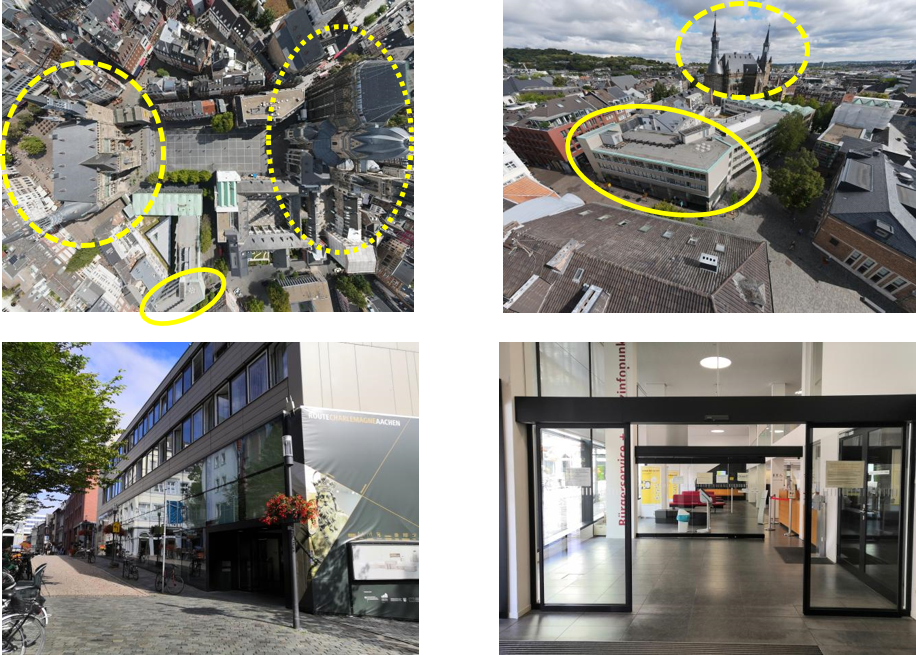
\includegraphics[width=\textwidth]{初来乍到/Bürgerservice/位于 Katschhof 的市政厅、Rathaus 和大教堂.png}
      \caption{位于 Katschhof 的市政厅、Rathaus 和大教堂。实线:\textsbf{市政厅/Bürgerservice Katschhof};虚线:\textsbf{Rathaus Aachen/City Hall Aachen};点线:\textsbf{大教堂/Aachener Dom/Aachen Cathedral}。}
      \label{fig:位于 Katschhof 的市政厅、Rathaus 和大教堂}
    \end{figure}

    \begin{figure}[ht]
      \centering
      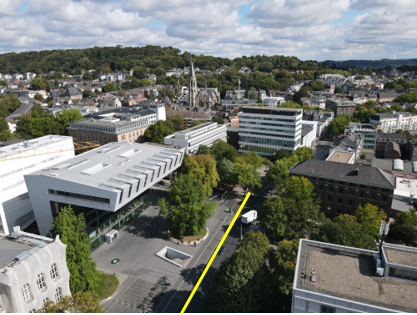
\includegraphics[width=.3\textwidth]{初来乍到/Bürgerservice/SuperC 和 Templergraben.png} \ 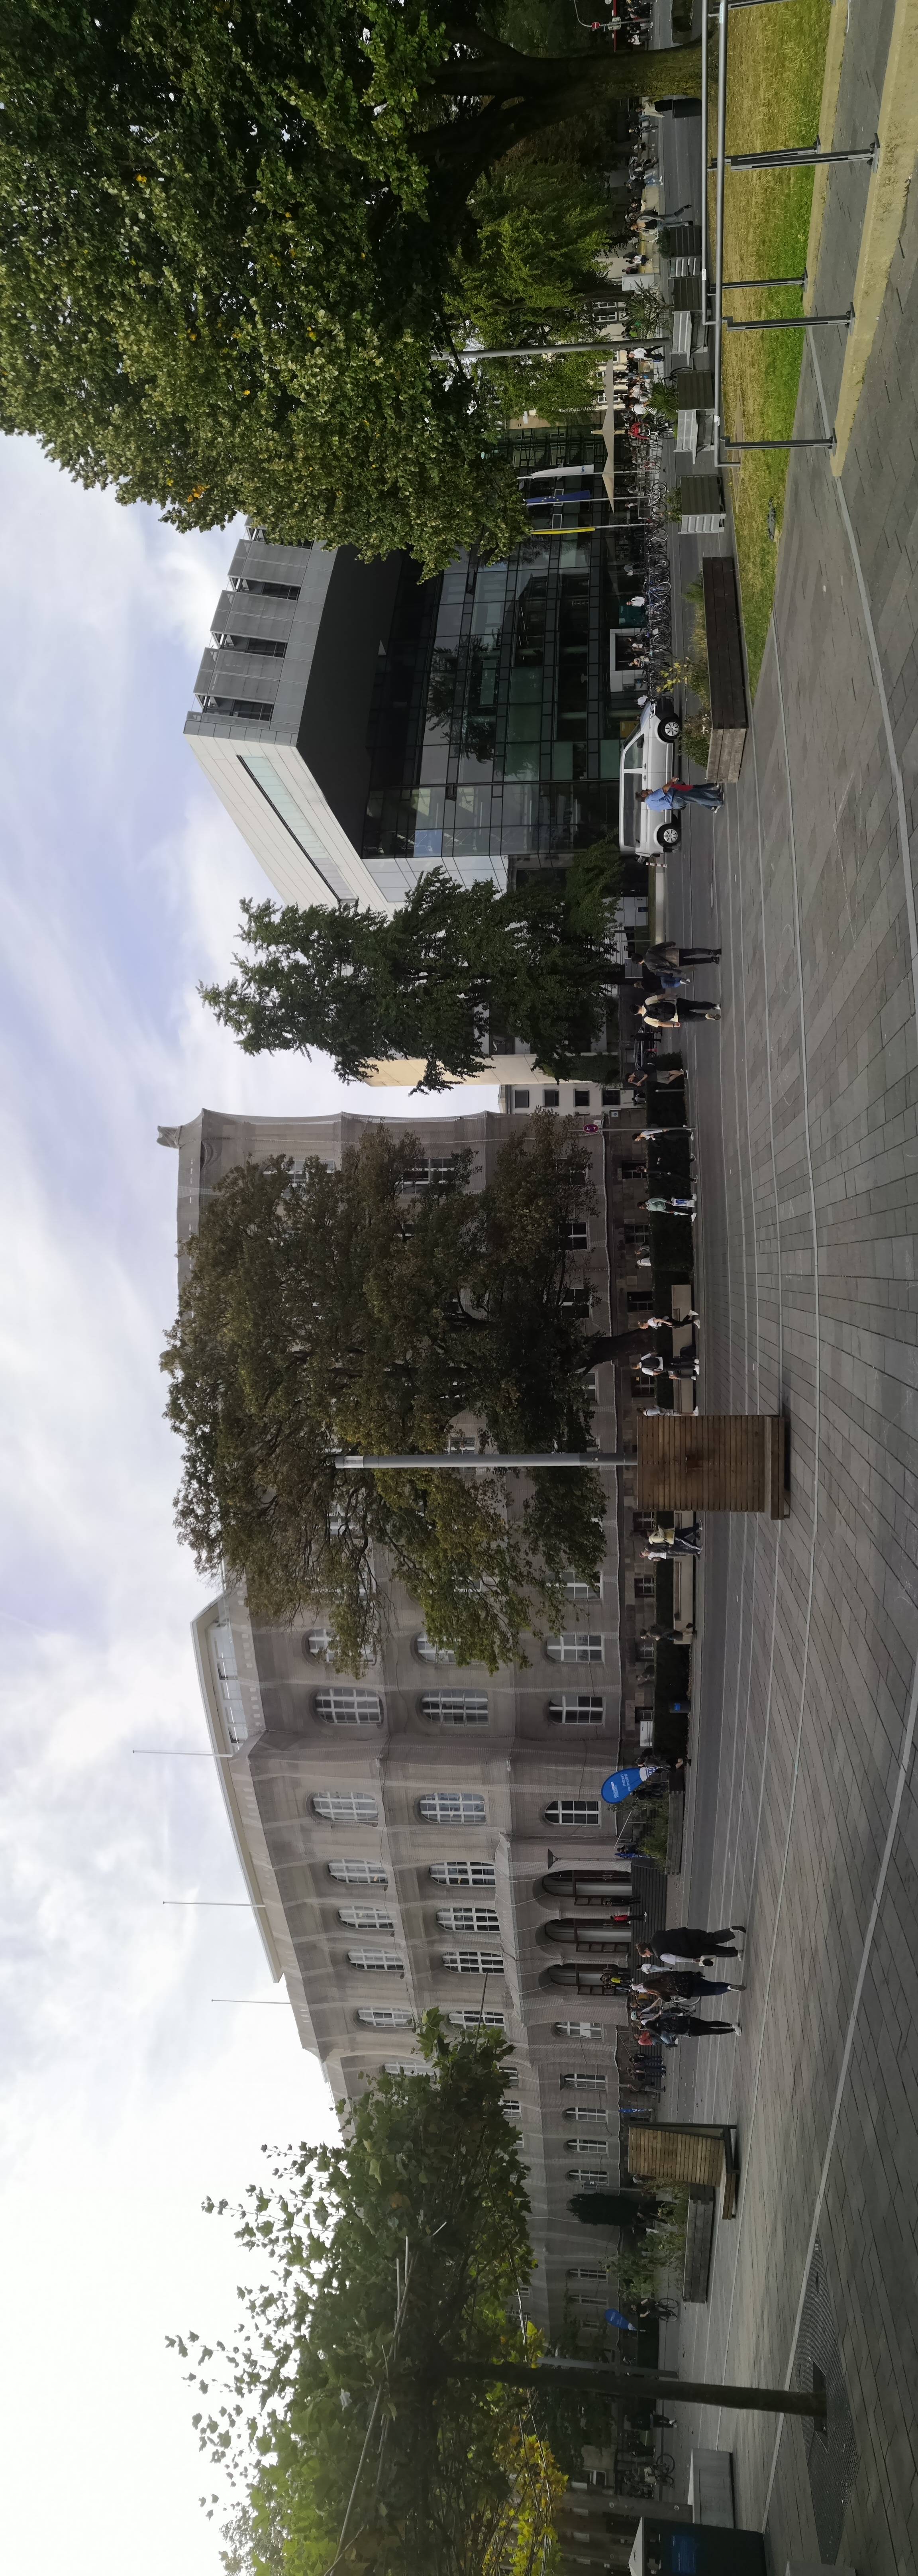
\includegraphics[width=.65\textwidth]{初来乍到/Bürgerservice/SuperC 和 Hauptgebäude.jpg}
      \caption{位于 Templergraben (黄线) 一侧的 \textsbf{SuperC} (右图右侧建筑) 和 \textsbf{主楼/Hauptgebäude} (右图左侧建筑)。}
      \label{fig:SuperC、Templergraben 和 Hauptgebäude}
    \end{figure}

    \begin{figure}[ht]
      \centering
      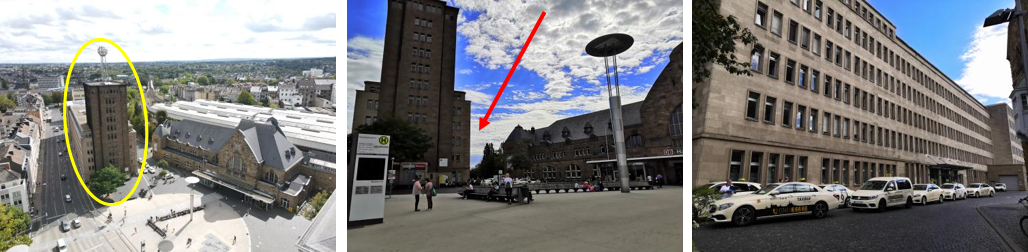
\includegraphics[width=\textwidth]{初来乍到/Bürgerservice/外管局.png}
      \caption{外管局/Ausländeramt}
      \label{fig:外管局/Ausländeramt}
    \end{figure}

\section{入境两周内必办事宜}\label{sec:入境两周内必办事宜}

  购买电话卡和办理宽带,签订租房合同以及Anmelden,银行卡激活,医保激活。这些都是您入境德国后要尽快落实的事情。有了Anmelden才能办理银行和医保的激活业务,您才可以使用德国的银行卡里的欧元进行消费,有了医保才能入学注册\footnote{即使您用的是N26银行,可以在无 Anmelden 的情况下使用在国内一次性打进来的12,324欧,但申请公保是需要固定住所的。}。

  每次更换地址 (找到了可 An 房) 后都要在银行和医保系统更换地址,以免纸质信件丢失。

  \subsection{电话卡和宽带}\label{subsec:电话卡和宽带}

    德国的几家大型网络运营商是\href{https://www.vodafone-shops.de/aachen-203344151/}{Vodafone}、\href{https://shopseite.telekom.de/west/aachen/holzgraben-6}{Telekom}、\href{https://www.o2online.de/shops/aachen/3}{o2}、e-puls等等;更多选择可以从\href{https://www.dazhe.de/}{德国打折网}查询。上网输入关键词搜索即可查询附近的服务点,购买电话卡和办理宽带。

    不同运营商的套餐和服务略有不同,常见的有prepaid和contract两类。简单解释是,前者可自由选择充钱与否,一般是从充钱之日算起一个月内有效,比较灵活;后者则类似于国内App的年付+续订,平均下来每个月比前者便宜。Vodafone有它对应的App叫Mein Vodafone,通过它可以线上充值,相对比较方便。

    所谓宽带是指租金里不含网费的、需要自行办理 WiFi 网络的那些住房 (Sec \ref{sec:住房})。有些公司同时办理电话卡和宽带 (DSL) 会有折扣。总之,您可根据自己的需要比较各个公司之间的套餐,在办理的时候可以咨询店员。

  \subsection{签订住房合同以及Anmelden}\label{subsec:签订住房合同以及Anmelden}

    关于签订合同的注意事项已经在 Sec \ref{sec:住房} 谈及过了。当您拿到租房合同或 \textsbf{Wohnenbestätigung}之后最好在两周以内完成 Anmelden (并不要求入住了新房才可以 An),然后分别去银行和医保门店换地址。

    \textsbf{Bürgerservice Katschhof} 麻雀虽小五脏俱全,排队的人通常不会很多;\textsbf{Bürgerservice Bahnhofplatz} 的业务则比较集中,除了 Anmelden 业务外还包括申请居留许可 (Sec \ref{sec:申请居留许可})。

    需要带上的文件通常为\textsbf{护照}与\textsbf{住房合同}。事前最好先问问房东``我需要带哪些东西去Anmelden'':房东对Anmelden政策的了解会比本手册更清楚。

    去 Anmelden 时需要先在 Bürgerservice 大厅处拿号排队 (也可提前\href{https://www.qtermin.de/bahnhofplatzkatschhof}{网上预约})。

    回家之后记得在自己的门牌上贴上自己的名字,或要求房东更换公寓楼下的住户列表,确保快递员和信使找得到您的名字。

  \subsection{银行账户激活}\label{subsec:银行账户激活}

    在到达了亚琛、有了固定地址、办理了\textsbf{Anmelden的证明}以后,即可办理 Sperrkonto 和 Girokonto 的激活手续\footnote{在银行账户激活之前也可以用国内的\textbf{银联卡}在 ATM 机取款,是根据实时汇率从人民币扣款的。},详见 Sec \ref{subsec:德意志银行}\textasciitilde\ref{subsec:N26}。有了 Girokonto 的 IBAN 后即可在没有收到银行卡的情况下签订房租、医保、电话卡和宽带的自动扣款合同。如果您更换了地址,则需要去亚琛的对应\textsbf{支行/Filiale} 更改在银行注册的地址。

  \subsection{医保激活}\label{subsec:医保激活}

    关于医保,初次入境得解决两个事情:私保缴费和公保申请。

    直接在网上填写您的护照、住所和银行卡等信息即可办理保险;也可以去亚琛当地的TK或AOK门店通过工作人员办理。完成后会给您发确认邮件以及纸质信件,后者附带了医保证明 (用于入学注册) 以及医保卡。

    医保的扣款方式是自动扣款的。其实,有了Girokonto的IBAN码即可在没有收到银行卡的情况下签订自动扣款的合同。所以即使您还没有收到银行寄过来的卡,也可以完成本小节的所有步骤。

    如果您更换了地址,则需要去门店 (TK, AOK, …) 或对应官网更改在医保系统的地址。

\section{RWTH注册和管理系统}\label{sec:RWTH注册和管理系统}

  RWTH的``注册''分为入学注册和学期注册。在签订了公保合同以后,即可办理入学注册手续,与此同时您即可登录学校的学生管理系统管理您的各项事务。

  \subsection{入学注册}\label{subsec:入学注册}

    大学新生须按照\textsbf{录取通知书/Zulassung/Zu}\footnote{Zu 专用于指代德国大学的录取通知书,经历过学校申请的同学应该不会对这个词过分陌生。}上所写的时间到\href{https://www.rwth-aachen.de/go/id/pvd/lidx/1}{\textsbf{国际办公室/外办/International Office}} 注册。录取通知书上会指明注册需要的证件与材料,这其中通常包括 (请以录取通知书中的信息为准):
    \begin{enumerate}
      \item 护照
      \item 录取通知书
      \item 国内学校毕业证书的原件及翻译公证件
      \item 语言水平证书
      \item 医疗保险证明
      \item 若是转学,则需要之前学校的退学证明
      \item 如申请时未交登记照,则需要登记照一张
      \item 某些专业可能需要的GRE成绩
      \item Anmelden证明
    \end{enumerate}
    
    在外办完成注册后您会拿到外办开具的注册证明和一张银行转账单,转账注册费以完成注册。除此以外您还会拿到用于激活\textsbf{学生管理系统} (Sec \ref{subsec:学生管理系统}) 的Coupon,登录IdM Selfservice按提示激活您的系统,激活完成后您会看到自己的账号ab123456和8位字符 (大小写+数字) 的初始密码信息,并一定要记下来2。同时,上传一张个人照片以用于BlueCard,并及时更改您的住所信息。

    入学注册后您将会拿到\textsbf{学生证/蓝卡/BlueCard} 和ASEAG的\textsbf{学期票/Semesterticket} (Sec \ref{sec:交通}) 的邮寄件。

    在RWTH通行,您主要有两个号码:一个是蓝卡上显示的入学号/MATR.-NR. 12345,主要用于考试;另一个是用于登录学生管理系统的ab123456 (其中ab是您的名-姓缩写)。

  \subsection{学生管理系统}\label{subsec:学生管理系统}

    RWTH的学生管理系统几乎承包了这个学校的所有业务,如无意外几乎不必麻烦人工服务。

    \href{https://online.rwth-aachen.de/}{RWTHonline} (Fig \ref{fig:RWTHonline}) 负责的业务包含选课、报名考试\&查看成绩、打印在读证明\&成绩单 (其PDF档就已盖有学校公章)、语言中心报名、交学费等。

    \href{https://idm.rwth-aachen.de/selfservice}{IdM Selfservice} (Fig \ref{fig:IdM Selfservice}) 可由RWTHonline登入,该系统主要用来管理您的账号密码以及您的设备在全校的WiFi服务:只要您身边有个RWTH的建筑,即可连上学校的eduroam的WiFi。

    \href{https://moodle.rwth-aachen.de/}{RWTHmoodle} (Fig \ref{fig:RWTHmoodle}) 管理所有学习资料,包括教授的讲义、提交作业和接收批改等等。

    \href{https://play.google.com/store/apps/details?id=de.rwth_aachen.rz.rwthapp&hl=en}{RWTHApp} (Fig \ref{fig:RWTHApp}) 则管理课程表、图书馆借书、食堂菜谱 (Sec \ref{subsec:大学食堂 Mensa})、空教室查询等等。

  \subsection{学生邮箱}\label{subsec:学生邮箱}

    注册不久,您就可以登录 \href{https://mail.rwth-aachen.de/}{RWTHmail} 管理您的邮箱。邮箱格式为 \href{mailto:vorname.nachname@rwth-aachen.de}{vorname.nachname@rwth-aachen.de}。假设某用户姓张名伟,则邮箱为 \href{mailto:wei.zhang@rwth-aachen.de}{wei.zhang@rwth-aachen.de}。

    但是要注意,登录 \href{https://mail.rwth-aachen.de/}{RWTHmail} 所需的账号为 \href{mailto:ab123456@rwth-aachen.de}{ab123456@rwth-aachen.de},这里,ab123456 是入学注册 (Sec \ref{subsec:入学注册}) 时您领到的学生管理系统的账号;登录 \href{https://mail.rwth-aachen.de/}{RWTHmail} 的密码则是ab123456的对应密码。同样假设用户的名字是张伟,则登录账号为 \href{mailto:wz123456@rwth-aachen.de}{wz123456@rwth-aachen.de},而\textbf{不是}以 \href{mailto:wei.zhang@rwth-aachen.de}{wei.zhang@rwth-aachen.de} 登录。

    通过这个邮箱,您可以享受绝大部分的学生优惠,包括GitHub的学生包。联系教授和申请实习和工作的时候也尽量使用这个邮箱。该邮箱在您毕业之后可以一直保留和使用,但 \href{https://online.rwth-aachen.de/}{RWTHonline} 等账号会在毕业180天后注销。

    \begin{figure}[H]
      \centering
      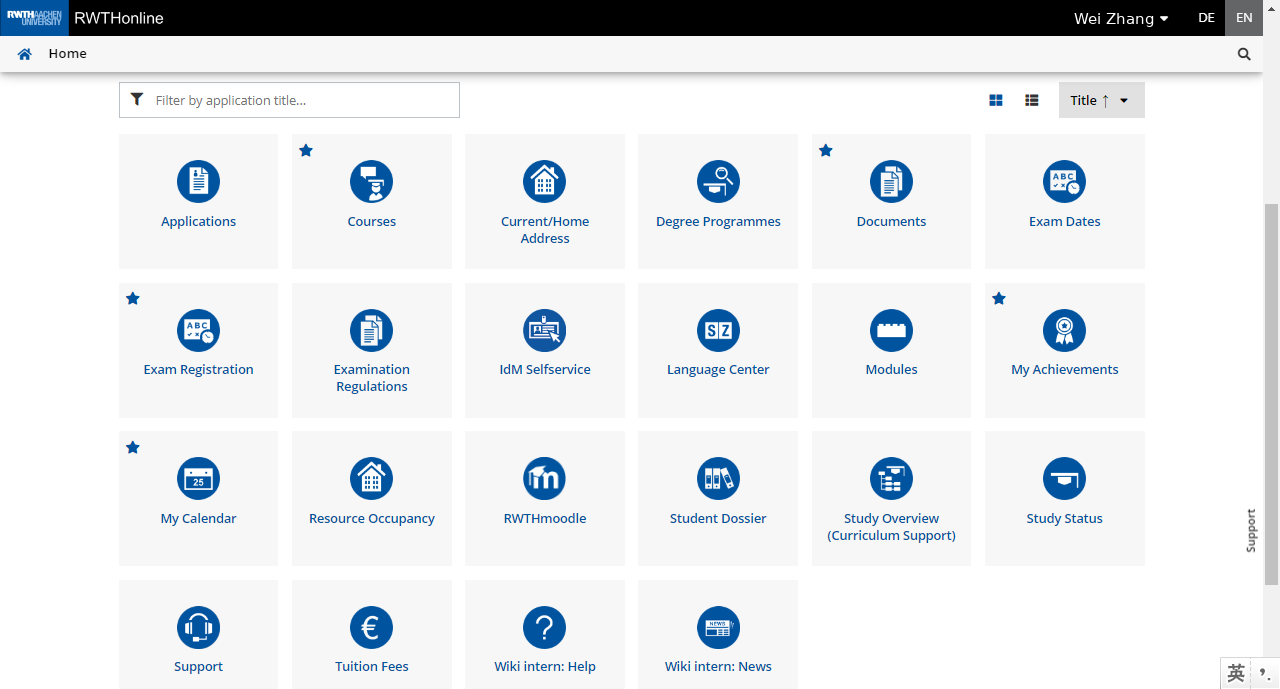
\includegraphics[width=\textwidth]{初来乍到/Management_System/RWTHonline.png}
      \caption{\href{https://online.rwth-aachen.de/}{RWTHonline}}
      \label{fig:RWTHonline}
    \end{figure}

    \begin{figure}[H]
      \centering
      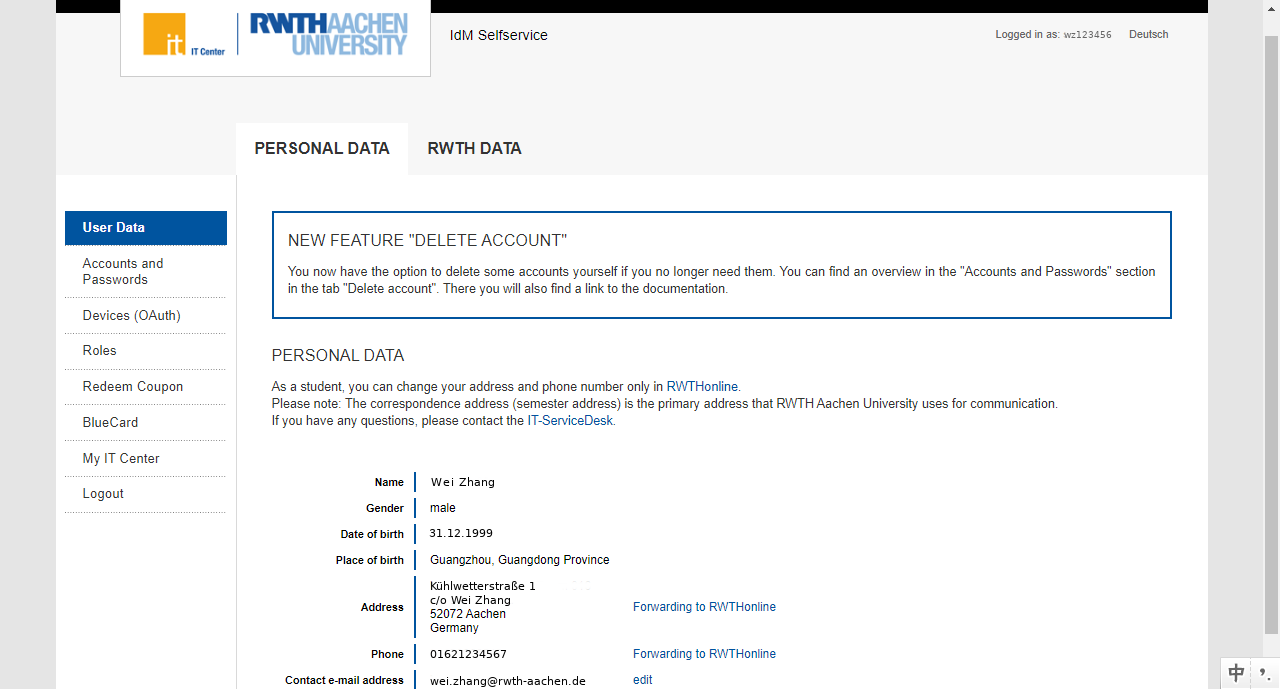
\includegraphics[width=\textwidth]{初来乍到/Management_System/idm.png}
      \caption{\href{https://idm.rwth-aachen.de/selfservice}{IdM Selfservice}}
      \label{fig:IdM Selfservice}
    \end{figure}

    \begin{figure}[H]
      \centering
      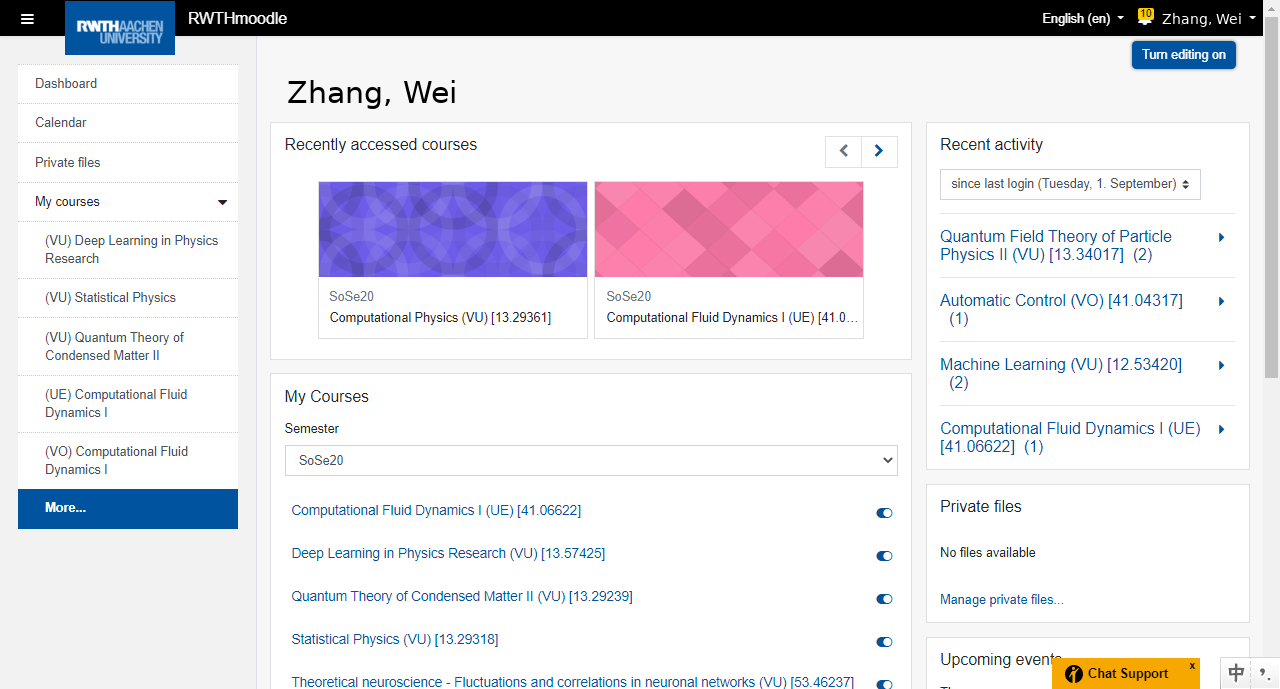
\includegraphics[width=\textwidth]{初来乍到/Management_System/RWTHmoodle.png}
      \caption{\href{https://moodle.rwth-aachen.de/}{RWTHmoodle}}
      \label{fig:RWTHmoodle}
    \end{figure}

    \begin{figure}[ht]
      \centering
      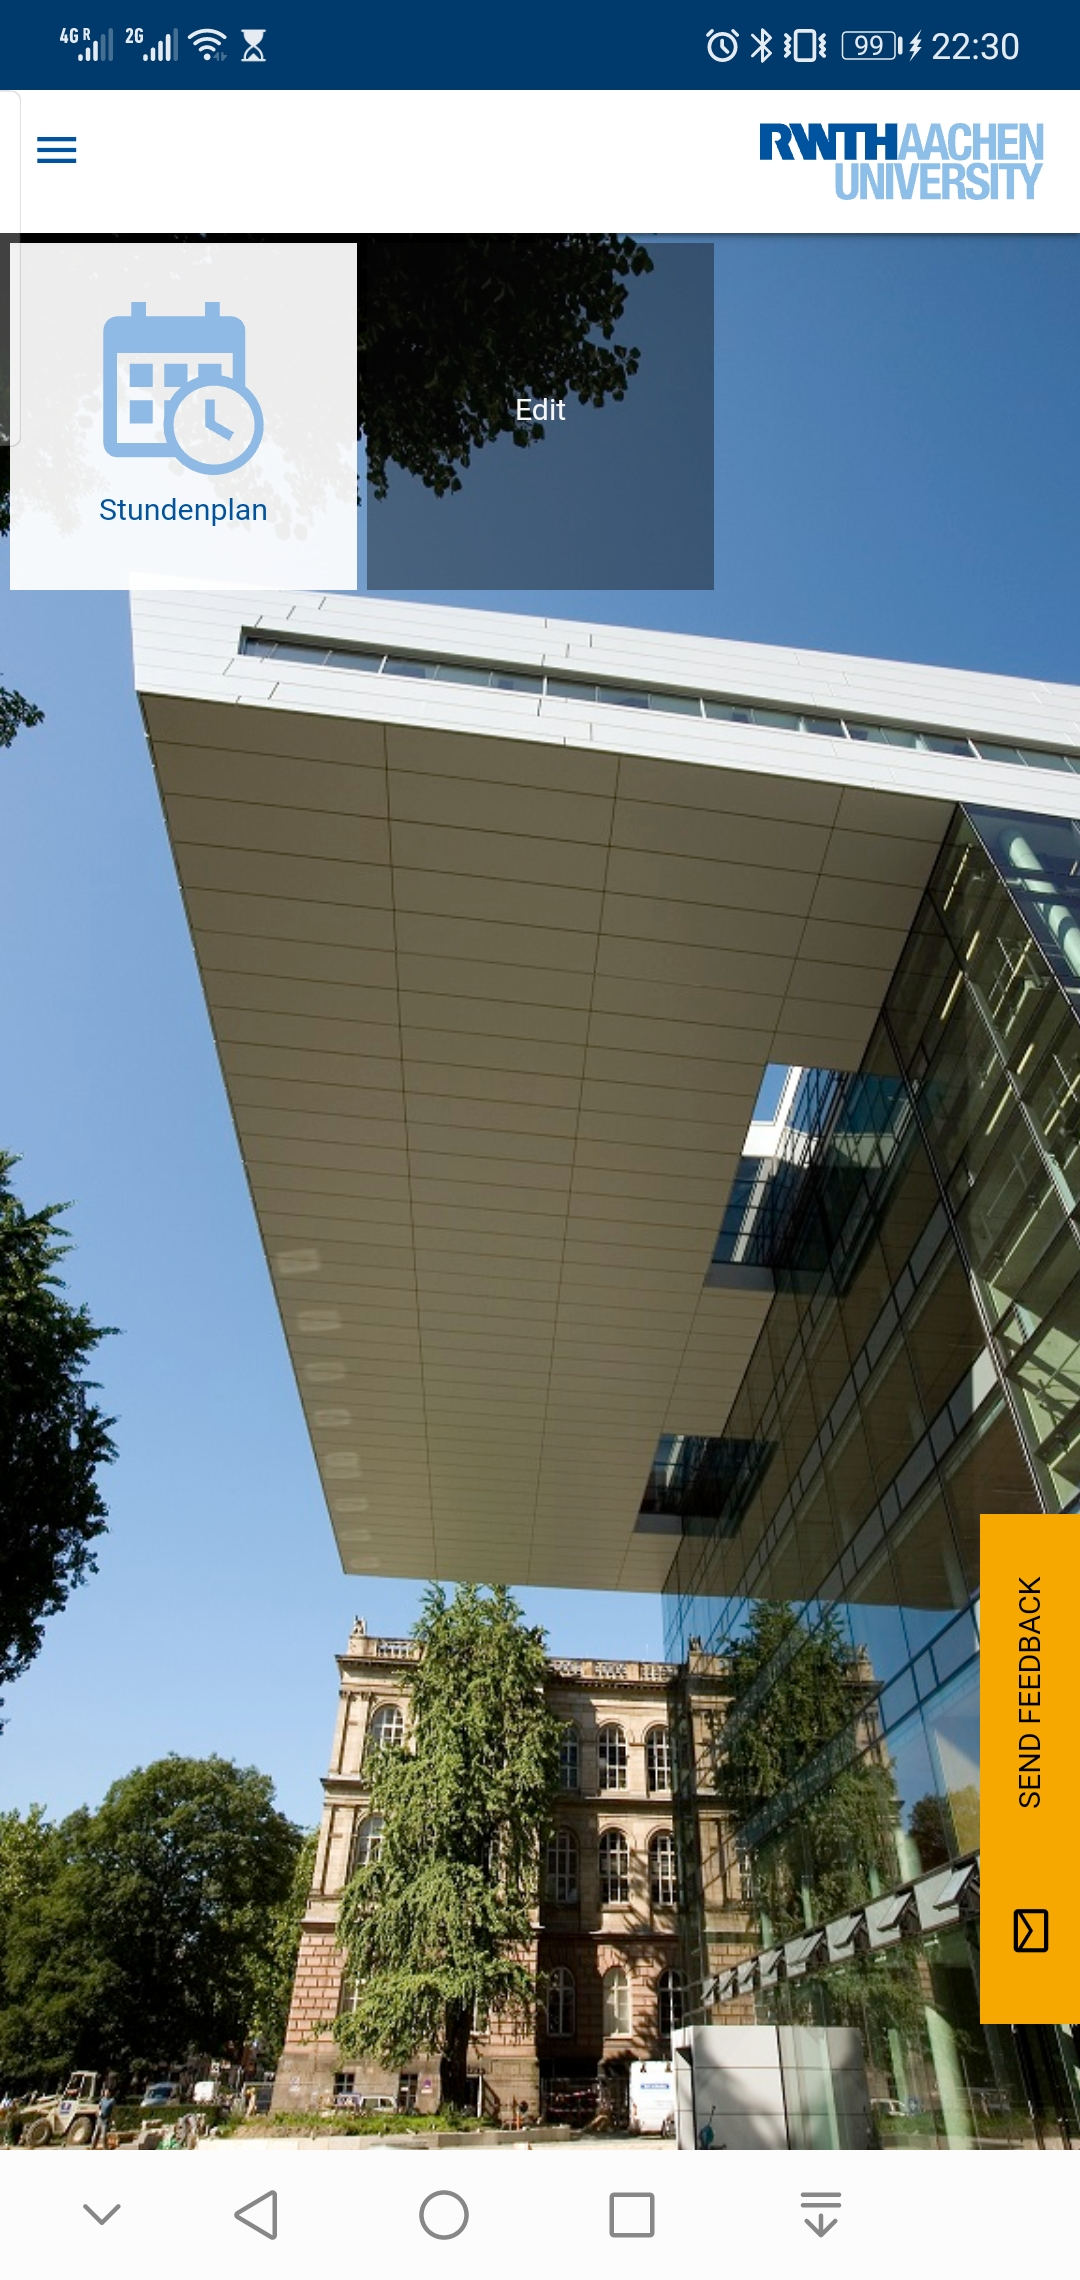
\includegraphics[width=.24\textwidth]{初来乍到/Management_System/RWTHApp_1.jpg} \ 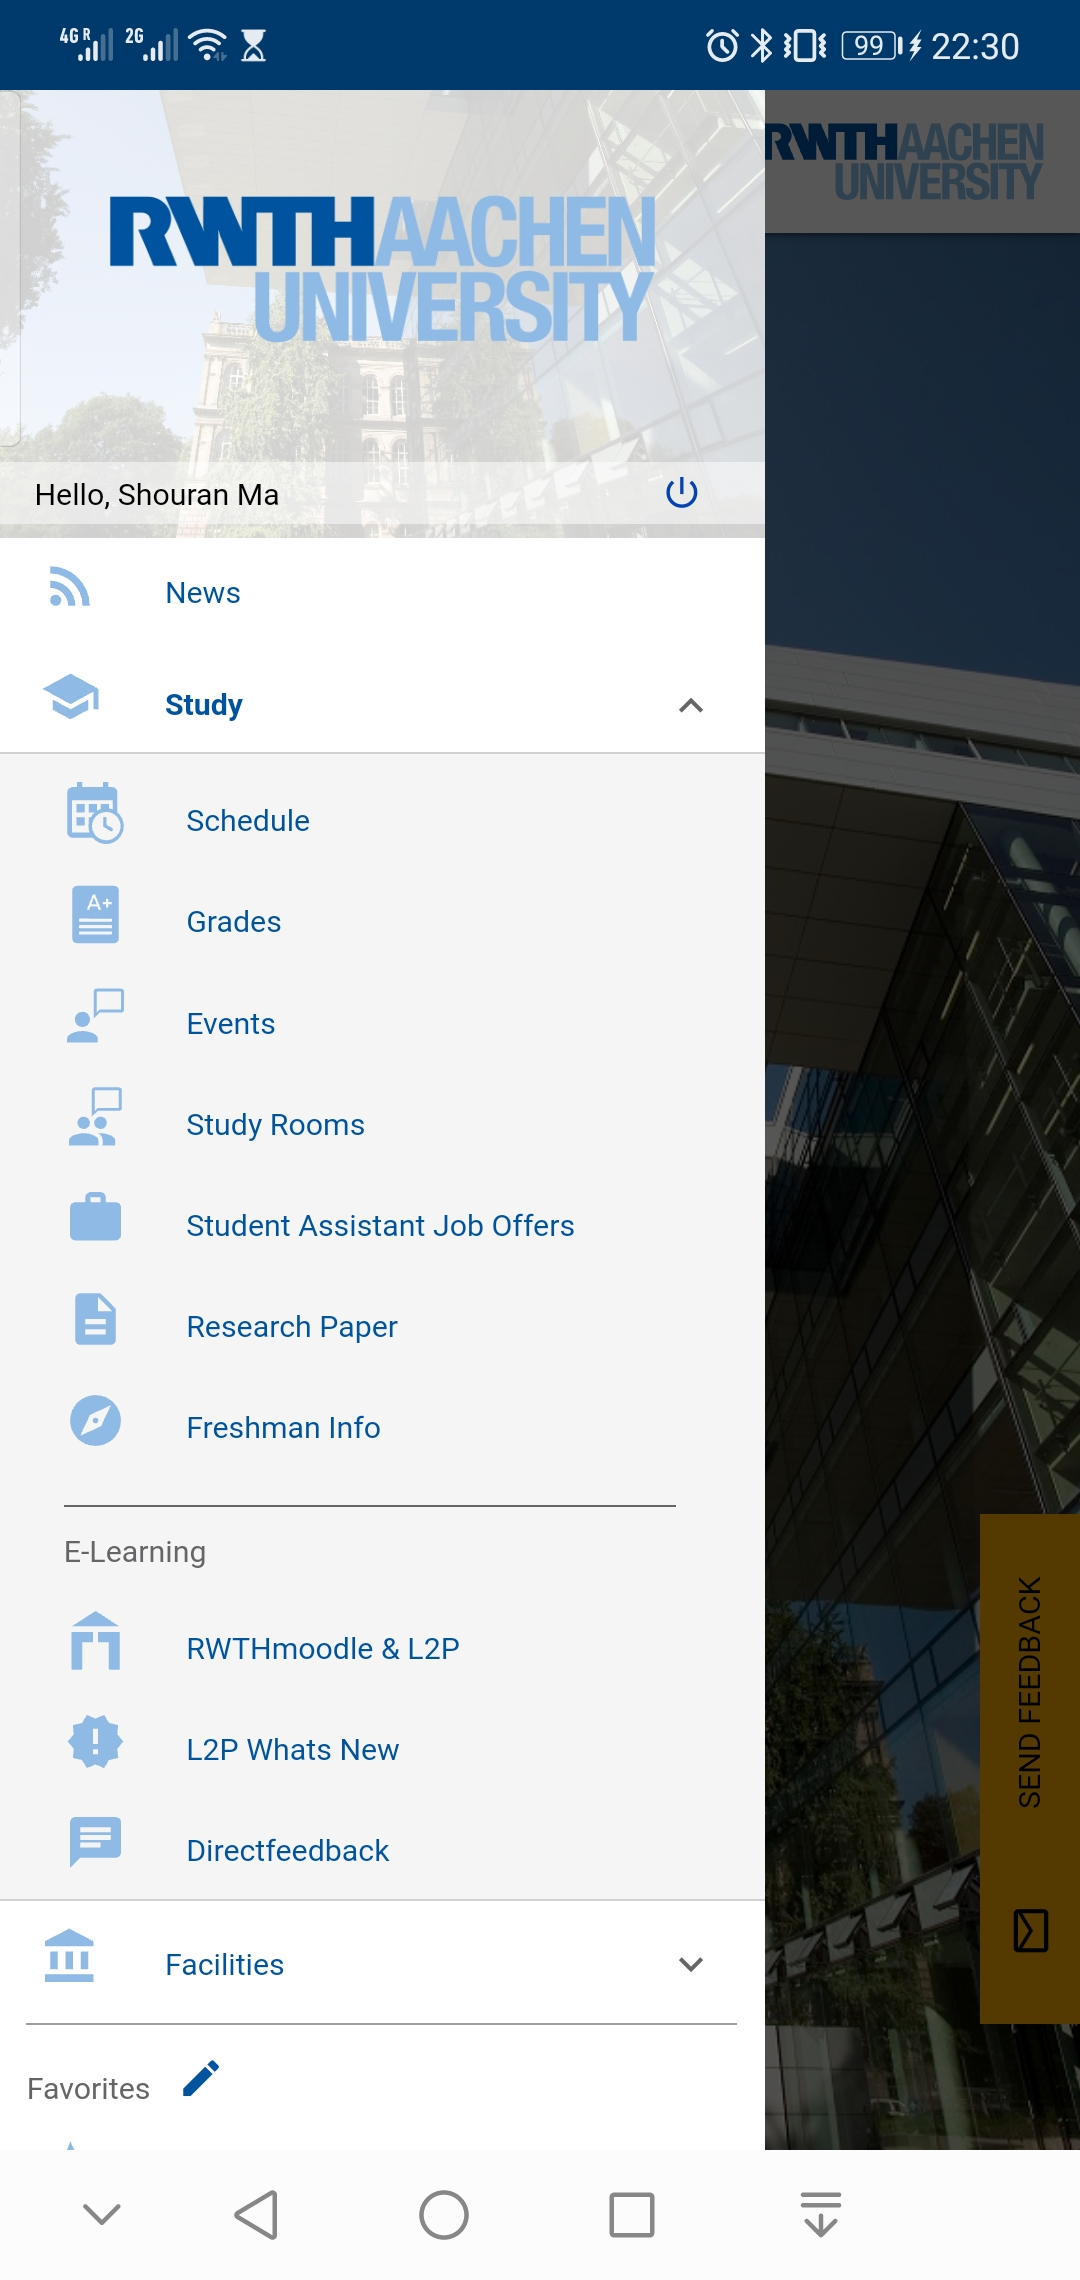
\includegraphics[width=.24\textwidth]{初来乍到/Management_System/RWTHApp_2.jpg} \ 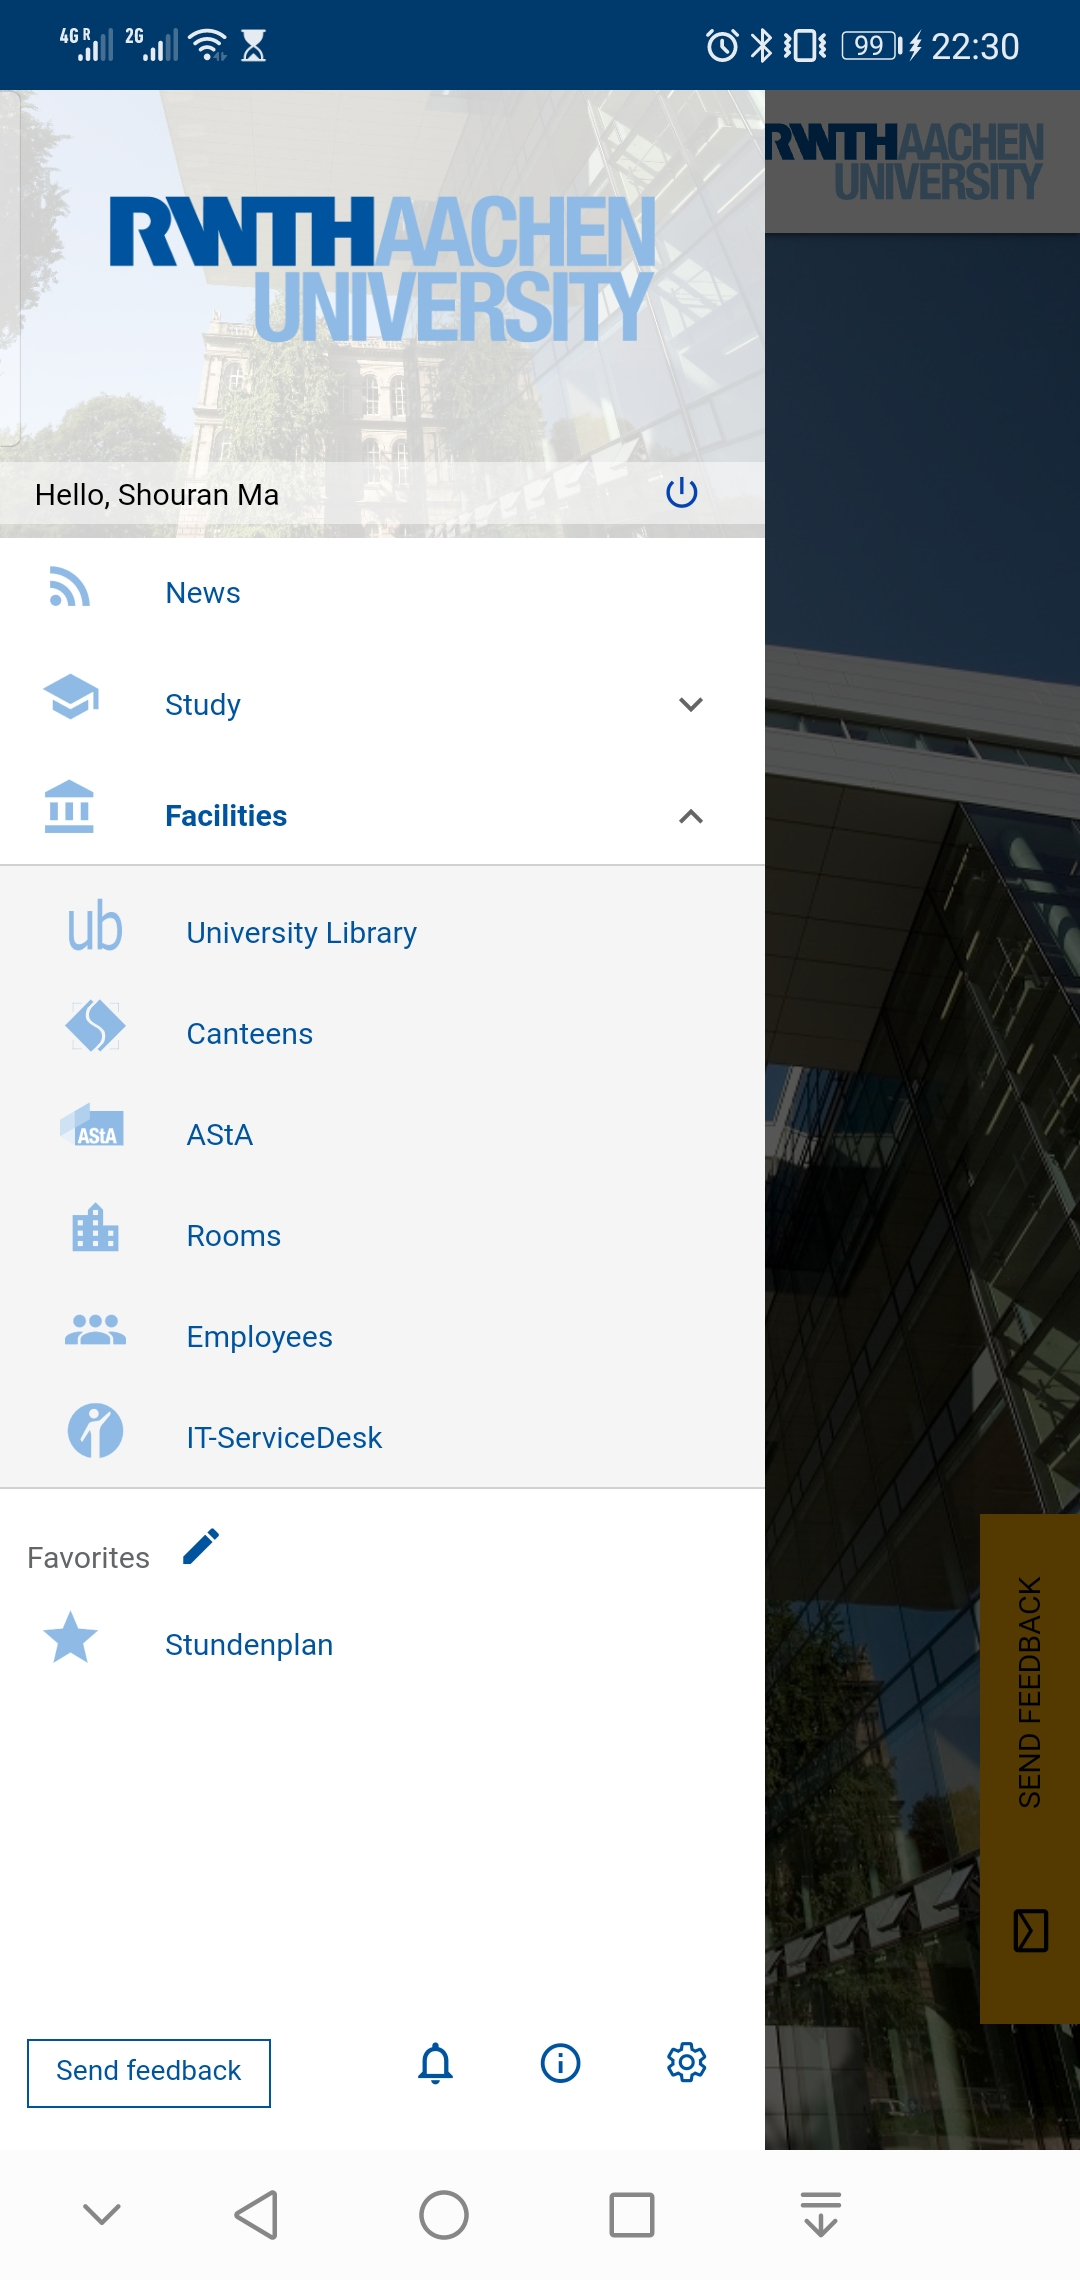
\includegraphics[width=.24\textwidth]{初来乍到/Management_System/RWTHApp_3.jpg} \ 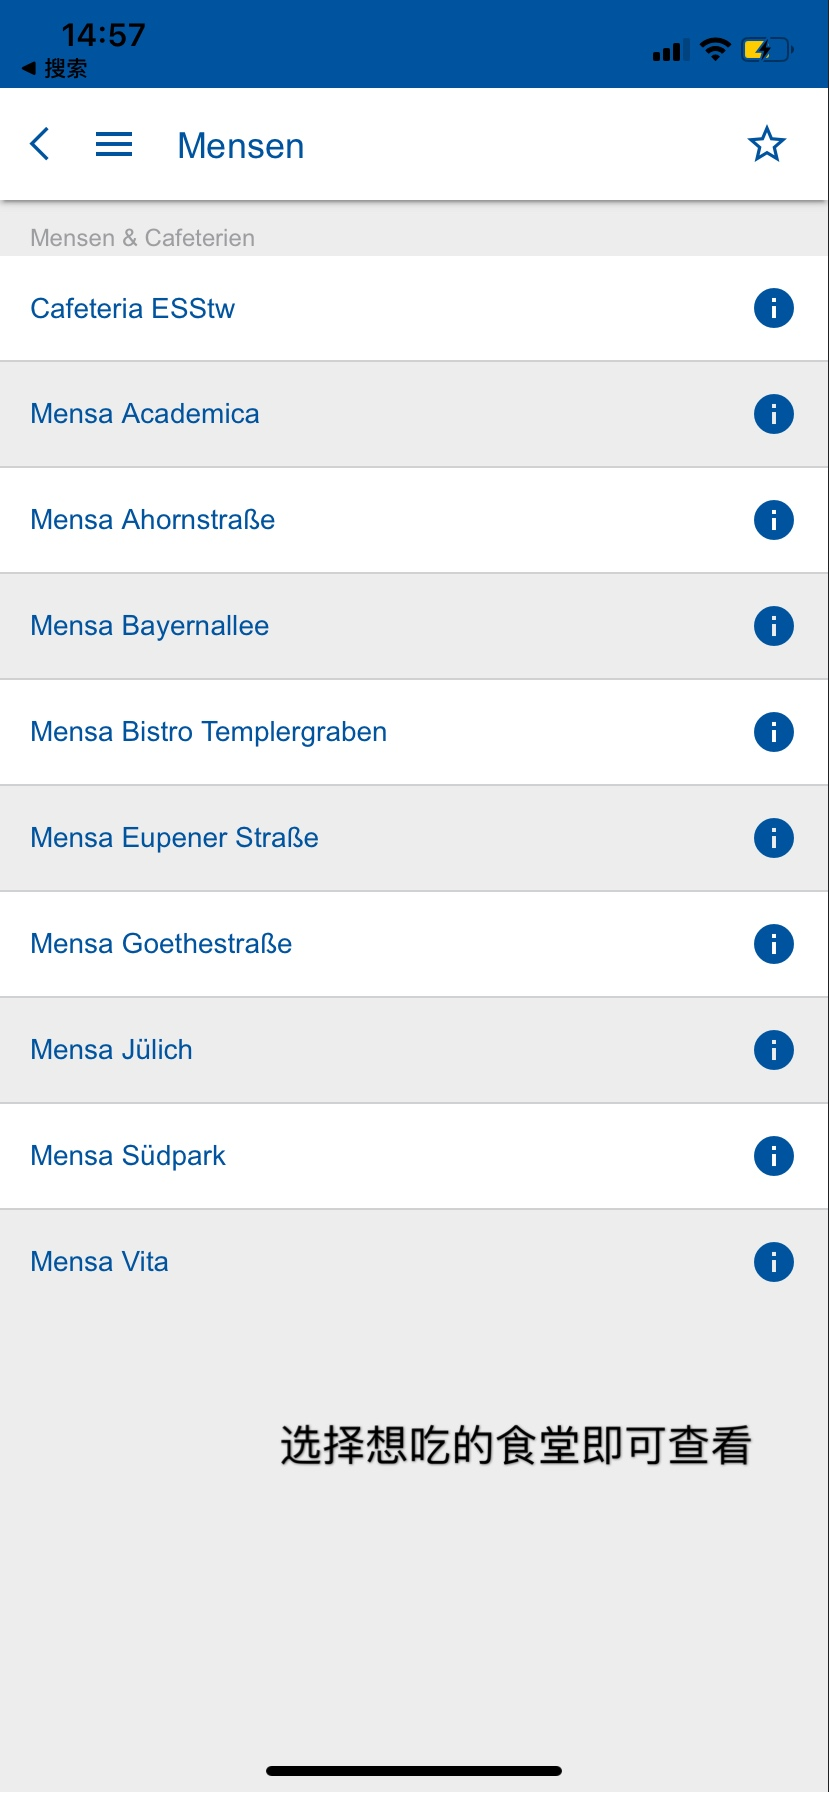
\includegraphics[width=.235\textwidth]{初来乍到/Management_System/RWTHApp_4.jpg}
      \caption{\href{https://play.google.com/store/apps/details?id=de.rwth_aachen.rz.rwthapp&hl=en}{RWTHApp}}
      \label{fig:RWTHApp}
    \end{figure}

\section{申请居留许可}\label{sec:申请居留许可}

  国内申请到的入境签证为六个月的\textsbf{学生签证}或为期三个月的的\textsbf{语言签证},都是短期签证。这个短期签证到期前一至两个月需要办理\textsbf{居住许可/居留卡/Aufenthaltstitel}的申请手续获得\textsbf{长期签证}。申请分为三步:\textbf{网上预约申请居留许可的 Termin},\textbf{Termin 当日递交材料}和\textbf{取卡},都在 \href{https://termine.staedteregion-aachen.de/auslaenderamt/}{StädteRegion Aachen} 上预约。

  \subsection{预约 Termin}\label{subsec:预约 Termin}

    主要有两个地方预约:

    \begin{itemize}
      \item SuperC: StädteRegion Aachen \MVRightarrow{} Aufenthaltsangelegenheiten \MVRightarrow{} RWTH - Außenstelle Super C \MVRightarrow{} RWTH Studenten;
      \item 主火旁的外管局 (Fig \ref{fig:外管局/Ausländeramt}):StädteRegion Aachen \MVRightarrow{} Aufenthaltsangelegenheiten \MVRightarrow{} Aufenthalt 根据姓氏选择。
    \end{itemize}

    \textbf{该网站在每日 0:00-0:10 之间开放申请。} 能够预约到 Termin 的日期通常在申请成功之日的1\textasciitilde2个月之后,所以在距离\textbf{居留许可到期的前1\textasciitilde2个月}就要及时在网站上刷号。当日的号在零点时分就会被全部申请完,在其他时间段是没有的,所以请坚持刷号。

    通常,外管局的延签比较容易约 Termin,但是两个地点并不是随意选取的。基本判断依据是,\textbf{如果您之前没有在别的城市延签过,就不需要调档案,可以直接去 SuperC 延签;如果有在别的城市延签过,外管局就需要从别的城市调取档案到亚琛,就需要去外管局延签}。对于后者的情况,外管局延签后,您的档案会被送到 SuperC,之后的延签就\textbf{应该}约 SuperC 的 Termin 而不应该约外管局的,否则,那里的工作人员不予延签,并会让您重新申请一个 SuperC 的 Termin,这又是一个艰难的刷号过程。

    去 SuperC 延签是绝大多数的情形:

    \begin{itemize}
      \item 从国内来 RWTH \textbf{直接}读本科/硕士,包括先修读语言班再入学以及直接入学的情形。
      \item 从\textbf{时长为半年的入境签证}转为\textbf{首次申请长期签证 (通常一年及以上)} 以及往后的\textbf{延签},都在 SuperC;
      \item 学分尚未修满,须延签。
    \end{itemize}

    而去约外管局 Termin 的则通常是如下情形:

    \begin{itemize}
      \item 若您是读预科的同学,须直接去外管局办理申请业务。
      \item 对于读预科的同学,当您已经成为或即将成为 RWTH 的学生后,依然先去外管局办理延签申请。外管局的工作人员发现您已是 RWTH 的学生了,他们就会把您的档案转给 RWTH 的签证办公室,这样下一次您就可以直接去学校延签了。
      \item 若之前\textbf{在德国其他城市}申请过签证或有过延签,则\textbf{首次在亚琛}办理改签/延签也需要在外管局办理。
    \end{itemize}

    关于申请,有如下 FAQ,部分摘自作者与 Ausländeramt 的工作人员的通讯,由于也是新生群里经常被问到的问题,故摘录于此:

    \begin{itemize}
      \item 如果我的居留许可即将 (在1\textasciitilde2周内) 到期但一直申请不上,怎么办?\\
      答:请给 \href{mailto:info.auslaendische.studenten@staedteregion-aachen.de}{info.auslaendische.studenten@staedteregion-aachen.de} 发邮件说明情况\footnote{这种情况,工作人员是会秒回邮件的,并不会像传言中的一个月才回复。}。工作人员是会认可这是及时的申请 (rechtzeitige Antragstellung)。但工作人员也表示,除了在 \href{https://termine.staedteregion-aachen.de/auslaenderamt/}{StädteRegion Aachen} 申请之外,并没有其他途径。
      \item 我申请到的 Termin 在居留许可到期日之后,在这期间我可以合法地在德国居留吗?\\
      答:请给 \href{mailto:info.auslaendische.studenten@staedteregion-aachen.de}{info.auslaendische.studenten@staedteregion-aachen.de} 发邮件说明情况。只要有这封邮件,这段时间在德居留依然被认为是合法的。但在这期间请务必不断地在 \href{https://termine.staedteregion-aachen.de/auslaenderamt/}{StädteRegion Aachen} 上刷号。
      \item 在旧居留许可到期日到新居留许可领取日之间我可以出国 (含回中国) 旅行吗?\\
      答:这需要 \textsbf{Fiktionsbescheinigung},俗称\textsbf{白条}。在 SuperC 的签证办公室 (Sec \ref{subsec:RWTH 的职能部门}) 的上班时间前往办理即可,无需预约。但是建议在这段时间非必要不旅行。
      \item 我持入境签证 (时长半年) 可以去周边国家旅行吗?\\
      答:原则上申根签证是在获得居住许可之后才会取得。所以,仅持入境签证是不可以去周边国家旅行的。
      \item 在哪里可以拍摄符合签证规格的照片?\\
      答:亚琛各大 DM (Sec \ref{subsec:线下商店-德国超市}) 以及\textsbf{Aachener Dom} (Fig \ref{fig:位于 Katschhof 的市政厅、Rathaus 和大教堂}) 附近的 \textsbf{Photo House Preim GmbH}。经验丰富的工作人员会根据照片用途 (用于德国的或其他欧盟国家的) 对照片进行裁剪。
    \end{itemize}

    申请成功并收到确认邮件以后,在指定日期携带材料前往指定地点提交。

  \subsection{递交材料}\label{subsec:递交材料}

    须提交的材料包括:
    \begin{enumerate}
      \item \href{https://bportal.staedteregion-aachen.de/staedteregion-a-z/-/egov-bis-detail/dienstleistung/15000/show}{申请表} (请务必区分\textsbf{首次申请/Erstantrag} 和 \textsbf{延签/Verlängerungsantrag});
      \item 护照 和 (上一次的) \textsbf{居留许可/elektronische Aufenthaltserlaubnis} + \textsbf{Zusatzblatt};
      \item 近期照片 (35mm*45mm);
      \item \textsbf{在读证明/Studienbescheinigung}:在 RWTHonline (Sec \ref{subsec:学生管理系统} Fig \ref{fig:RWTHonline}) Documents 下载打印;
      \item 收入证明 (每月至少934欧):如奖学金证明,近三个月的银行流水,雇佣合同,等 (请在 \href{https://www.auswaertiges-amt.de/de/sperrkonto/375488}{Auswärtiges Amt} 查询欲延长至少一年期签证所需的自保金额度;2023年的数据是11,208欧);
      \item 医疗保险证明:前往您所办理的公保公司驻亚琛办公室 (Sec \ref{sec:医疗保险}) 开具 (不可使用医保卡代替);
      \item PhD 学生须提供雇佣合同。
    \end{enumerate}
    所需费用:首次申请长期签证费用100欧,延签费用93欧;\textsbf{Fiktionsbescheinigung}时长半年,费用 13 欧。

  \subsection{取卡}\label{subsec:取卡}

    大约1个月以内,您就会收到\textbf{一封}标题为 \textsbf{elektronischer Aufenthaltstitel} 的\textbf{纸质信函},上面有对应您本次居留许可的 \textsbf{Transport-PIN} 和 \textsbf{PUK}。收到该信以后就可以在 \href{https://termine.staedteregion-aachen.de/auslaenderamt/}{StädteRegion Aachen \MVRightarrow{} Aufenthaltsangelegenheiten \MVRightarrow{}  Abholung \MVRightarrow{} Abholung Aufenthaltserlaubnis} 约 Termin。取卡的 Termin 则很充裕,全天任何时候都能申请。如今取\textsbf{居留许可/elektronische Aufenthaltserlaubnis}和\textsbf{Zusatzblatt}的是在\textsbf{Rothe-Erde Bahnhof}对面不远处的\textsbf{Aachen Arkaden}。

  \subsection{找工作签证}

    虽然毕业生不算是``新生'',但我们也把毕业找工作以及相关签证 (所谓``找工作签证'',\textsbf{arbeitsplatzsuche}) 的事宜列在这里,因为这事在新生群里也是被频繁问到的。

    相关重要流程包括:
    \begin{center}
      向ZPA交论文 \MVRightarrow{} 答辩 \MVRightarrow{} 论文出成绩 \MVRightarrow{} 领毕业证 \MVRightarrow{} 递交``找工作签证''的申请材料
    \end{center}
    提交的材料里\textbf{必须包含}\textsbf{毕业证}。可以加上简历、动机信、接收信、面试邀请等内容,但不是必须\footnote{从中国到德国境内的``找工作签证''是需要这些材料的,如\href{https://china.diplo.de/blob/1341662/3467e6cb74888d4cb9d8e188c4f4308b/pdf-merkblatt-natvisum-arbeitsaufnahme-data.pdf}{德国驻华使领馆 \MVRightarrow{} 服务 \MVRightarrow{} 签证和入境 \MVRightarrow{} 长期停留 \MVRightarrow{} 德国工作签证申请须知}。}。德国政府也是希望在德国高校毕业的学生能留在德国工作,就业环境比较宽松,所以\textbf{找工作签证从 12 到 18 个月不等}。

    通常,在提交毕业论文到论文出成绩就有 8 周的时间。此外,不少研究组织和公司虽然在招聘信息里写着``需要提交毕业证'',实际上在毕业论文的末期也可以申请。这些时间加起来足够去写申请信和找工作了。

    此外有一种情形是,您已经通过面试且有意向入职,但有不少杂事,如工作单位开具合同,那么申请 Fiktionsbescheinigung 也是可以的。
